\PassOptionsToPackage{svgnames}{xcolor}
\documentclass[11pt,a4paper]{article}
\usepackage[utf8]{vietnam}
\usepackage[dvipsnames]{xcolor}
\usepackage{pgfplots}
\pgfplotsset{grid style={dashed,gray}}
\pgfplotsset{major grid style={dashed,gray}}
\usepackage{graphicx}
\usepackage{tikz}
\usepackage{lettrine}
\usepackage[object=vectorian]{pgfornament} %%  http://altermundus.com/pages/tkz/ornament/index.html
\usepackage{lipsum}
\usetikzlibrary{calc}
\usepackage[top=2cm, bottom =2cm, right=2cm, left=2cm]{geometry}
\usepackage{algorithm}
\usepackage[noend]{algpseudocode}
\usepackage{amsmath}
\thispagestyle{empty}
\usepackage{transparent}
\usepackage{eso-pic}
\usepackage{enumitem}
\usepackage{xfrac}
\usepackage{graphicx}
\usepackage{multicol}
\usepackage{graphics}
\usepackage{tabularx}
\usepackage{titletoc}
\usepackage{float} %fix positioning image 
\algdef{SE}[DOWHILE]{Do}{doWhile}{\algorithmicdo}[1]{\algorithmicwhile\ #1}%
\newcommand\BackgroundPic{%
\put(0,0){%
\parbox[b][\paperheight]{\paperwidth}{%
\vfill
\centering
{\transparent{0.2} 
\includegraphics[width=\paperwidth,height=\paperheight,%
keepaspectratio]{Logo_hcmus.png}}%
\vfill
}}}
\newcommand{\sectionline}{%
  \noindent
  \begin{center}
  {\color{Black}
    \resizebox{0.7\linewidth}{1ex}
    {{%
    {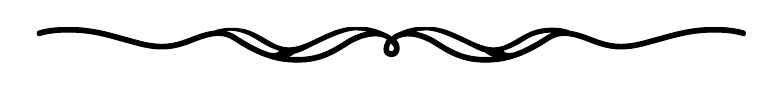
\begin{tikzpicture}
    \node  (C) at (0,0) {};
    \node (D) at (9,0) {};
    \path (C) to [ornament=85] (D);
    \end{tikzpicture}}}}}%
    \end{center}
}
%% A macro with two arguments to change ornaments and colors easily
%% Syntax -- \sectionlinetwo{<color>}{<ornament>}
\newcommand{\sectionlinetwo}[2]{%
  \nointerlineskip \vspace{.5\baselineskip}\hspace{\fill}
  {\color{#1}
    \resizebox{0.8\linewidth}{2ex}
    {{%
    {\begin{tikzpicture}
    \node  (C) at (0,0) {};
    \node (D) at (9,0) {};
    \path (C) to [ornament=#2] (D);
    \end{tikzpicture}}}}}%
    \hspace{\fill}
    \par\nointerlineskip \vspace{.5\baselineskip}
  }
  
\usepackage{tocloft}

\advance\cftsecnumwidth 0.5em\relax
\advance\cftsubsecindent 0.5em\relax
\advance\cftsubsecnumwidth 0.5em\relax
  
%\renewcommand{\thesection}{\Roman{section}.} 

\usepackage{hyperref}
\hypersetup{hidelinks}
%\hrefstyle{same}

\usepackage{tikz}
\usetikzlibrary{calc}
\usetikzlibrary{arrows}
\usepackage{pgfplots}

\begin{document}
\AddToShipoutPicture*{\BackgroundPic}
\ClearShipoutPicture
\begin{tikzpicture}[remember picture,overlay]
  \draw[line width = 1pt] ($(current page.north west) + (0.5in,-0.5in)$) rectangle ($(current page.south east) + (-0.5in,0.5in)$);
  \end{tikzpicture}
 \begin{center}

 \LARGE {\textbf{TRƯỜNG ĐẠI HỌC KHOA HỌC TỰ NHIÊN}} \\
 %\scriptsize{ĐẠI HỌC QUỐC GIA - THÀNH PHỐ HỒ CHÍ MINH} \\
 \large{\textbf{ĐẠI HỌC QUỐC GIA - THÀNH PHỐ HỒ CHÍ MINH}}\\[.2in]
 %\rule{4in}{0.01cm}

\sectionlinetwo{Black}{88}
 \vspace{2in}
 %
\includegraphics[scale=0.2]{Logo_hcmus.png}\\
 
 \Huge{\textbf{REPORT}}\\
 \vspace{.2in}
 \end{center}
 
\center{\textbf{\huge{SORTING ALGORITHMS:}} \vspace{0.1in}\\\Large{\textit{\textbf{IDEA, TIME PERFORMANCE, DATA ANALYSE}}}}
\vspace{1in}
\begin{flushleft}
\large{\textbf{\textit{GROUP MEMBERS:}}}
\end{flushleft}
\begingroup
\setlength{\tabcolsep}{10pt}
\renewcommand{\arraystretch}{1.2}
\LARGE
\begin{flushleft}
\begin{tabular}{l l l}
\textbf{21127403}  & \hspace{.1in} \textbf{Nguyễn Minh Quân}\\
\textbf{21127664}  & \hspace{.1in} \textbf{Trần Đại Niên}\\
\textbf{21127602}  & \hspace{.1in} \textbf{Nguyễn Hoàng Duy}\\
\textbf{21127718}  & \hspace{.1in} \textbf{Lưu Vĩnh Tuấn}\\
\end{tabular}\\
\end{flushleft}
\endgroup

\vspace{0.1in}

\begin{flushleft}
\large{\textbf{\textit{INTRUCTORS:}}}
\end{flushleft}

\begingroup
\setlength{\tabcolsep}{10pt}
\renewcommand{\arraystretch}{1.2}
\LARGE
\begin{center}
\begin{tabular}{l r}
\textbf{Văn Chí Nam} & \hspace{4cm} \textbf{Bùi Huy Thông} \\
\textbf{Lê Thanh Tùng}  & \hspace{4cm} \textbf{Trần Thị Thảo Nhi}\\
\end{tabular}\\
\end{center}
\endgroup
\vspace{.1in}

\sectionlinetwo{Black}{88}

\pagebreak
\captionsenglish{ 
	\tableofcontents
}
\pagebreak
\flushleft{
	\section{Introduction}
	The project is about doing research on some common  and basic sorting algorithms. We will learn about how each algorithm works, 
	how it performs with different order of data(random/ reversed sorted/ nearly sorted/ sorted array), 
	what its application in real life, some advantage and disavantage of each algorithm. With all the knowledge from these algorithm, we will make a application
	for the user to know what is the runtime and how many comparisons a specific algorithm takes to sort the whole array. The user can define the data range, the order of data then the data will 
	be generated automatically or using data from input file. User can ask program to return the output from one algorithm or two algorithm simultaneously.
	\\[12pt]Through this project, we have a oppoturnity to work as a group and practice reading research and take in some new knowledge and understand more
	about how the data is sorted in different ways. And with the support from our teachers, we are able to do the research more efficiently and know what need to be done in order to 
	accomplish our goals. So our group members are extremely thankful to our teacher: Dr. Van Chi Nam, Mr. Bui Huy Thong, Ms. Tran Thi Thao Nhi, Mr. Le Thanh Tung for putting so much 
	effort to help us to achieve our goals.
	\\[12pt]All the code is coded in C\texttt{++}. the report is written in \LaTeX  \hspace{1pt} and all references we used are mentioned in the reference section at the end of the report.
	\\[12pt]The experiment is conducted on Laptop with these Properties:
	\begin{itemize}
	    \item Operating system: Window 11 Home Single Language 64-bit  (10.0, Build 22000)
	    \item System manufacturer: Acer
	    \item System model: Nitro AN515-57
	    \item BIOS: V1.10
	    \item Processor: 11th Gen Intel(R) Core(TM) i5-11400H @ 2.70GHz(12 CPUs), ~2.7GHz
	    \item Memory: 8192MB Ram    
	\end{itemize}
	\pagebreak
	\section{Algorithm Presentation}
		\rule{15cm}{0.1cm}
		\centering \subsection{Selection Sort}
		\rule{15cm}{0.1cm}
			\begin{enumerate}[label=\textbf{\arabic*})]
				\item \textbf{Main idea:}
				
				The selection sort simply partition the list into two main logical parts, the sorted part and the unsorted part. Any iteration picks a value from the unsorted and places it in the sorted list, making the sort partition grow in size while the unsorted partition shrinks for each iteration. When adding to the sorted list, the algorithm makes sure that the value is added at the right position to ensure an order sequence of the sorted partition. The process is terminated when the number of items or the size of the unsorted is one (1). The procedure to select a value to be moved to the sorted list will return minimum value or maximum value in the unsorted partition, which will be swapped to position the item correctly. 
				\\[12pt]
				\item \textbf{Complexity Analysis of Selection Sort}
					
					Let’s say n is the number of elements in the array. 
					\\[9pt]
					\textbf{Time complexity}
					
					Selection sort has the time complexity $\mathcal{O}(n^2)$ in best, worst and average cases.
					
					\textbf{Best case:} occurs when there is no need for sorting, i.e. the array has already been sorted.
					
					\textbf{Worst case:} occurs when array elements must be sorted in reverse order. Assume you need to sort the array elements in ascending order, but they are in descending order.
					
					\textbf{Average case:} occurs when the array elements are arranged in a jumbled order that is neither ascending nor descending correctly.
					\\[9pt]
					\textbf{Space complexity:}
					
					Due to being an in-place sorting algorithm, the space complexity is $\mathcal{O}$(1).
				\\[12pt]
				\item \textbf{Pseudo code:}
				\begin{algorithm}
                \caption{Selection Sort}
                \begin{algorithmic}[1]
                \Procedure{Selection Sort}{$a,n$} 
                    \For {$i = 0 \textbf{ to } n-1$}
                		\State $min \gets i$
                		\For {$j = i+1 \textbf{ to } n$}
                			\If{$a[j]<a[min]$}
                				min = j
                			\EndIf
                		\EndFor
                		\If{$min \neq i$}
                			\State Swap(a[min], a[i])
                		\EndIf
                	\EndFor
                \EndProcedure
                \end{algorithmic}
                \end{algorithm}
				\\[12pt]
				\item \textbf{Flowchart:}
					\begin{figure}[H]
						\centering 
						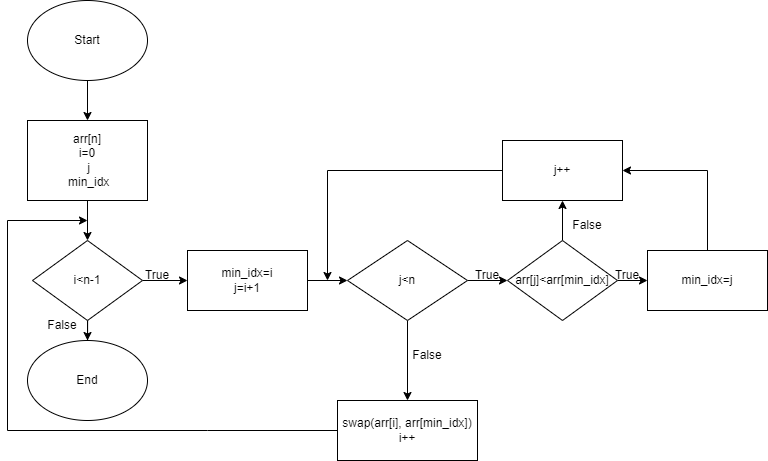
\includegraphics[width=0.6\textwidth]{SelectionSort Flowchart}
					\end{figure}
				
				\item \textbf{Description:}
					\begin{itemize}
						\item Find the smallest element in the array and swap it with the first element of the array i.e. a[0].
						\item The elements left for sorting are n-1 so far. Find the smallest element in the array from index 1 to n-1 i.e. a[1] to a[n-1] and swap it with a[1].
						\item Continue this process for all the elements in the array until we get a sorted list.
					\end{itemize}
				
				\item \textbf{Variants/ improvements:}
				
					\textbf{Heap sort}
					Heapsort greatly improves the basic algorithm by using an implicit heap data structure to speed up finding and removing the lowest datum. If implemented correctly, the heap will allow finding the next lowest element in $\mathcal{O}$log n time instead of $\mathcal{O}$(n) for the inner loop in normal selection sort, reducing the total running time to $\mathcal{O}$(n log n). Further information about Heapsort will be discussed later.
					
					\textbf{Cocktail sort}
					A bidirectional variant of selection sort, called cocktail sort, is an algorithm which finds both the minimum and maximum values in the list in every pass. This reduces the number of scans of the list by a factor of 2, eliminating some loop overhead but not actually decreasing the number of comparisons or swaps. 
					
					\textbf{Bingo sort}
					In the bingo sort variant, items are ordered by repeatedly looking through the remaining items to find the greatest value and moving all items with that value to their final location. This is an efficient variant if there are many duplicate values. Indeed, selection sort does one pass through the remaining items for each item moved. Bingo sort does one pass for each value (not item): after an initial pass to find the biggest value, the next passes can move every item with that value to its final location while finding the next value
				\item \textbf{Advantage, disadvantage:}
					\begin{table}[H]
						\centering
						\begin{tabular}{|p{8cm}|p{8cm}|}
							\hline
							\textbf{Advantage} & \textbf{Disadvantage} \\
							\hline
							\hline
							The main advantage of the selection sort is that it performs well on a small list. 							 											& The primary disadvantage of the selection sort is its poor efficiency when dealing with a huge list of items. \\[12pt]
							Because it is an in-place sorting algorithm, no additional temporary storage is required beyond what is needed to hold the original list. 				& The selection sort requires an n-squared number of steps for sorting n elements. \\[12pt]
							\vspace{12pt}
							Its performance is easily influenced by the initial ordering of the items before the sorting process. 													& \\[12pt]
							\vspace{12pt}
							Can be useful when memory write is a costly operation.  																								& \\
							\hline
						\end{tabular}
					\end{table}
				\item \textbf{Application:}	
					Used in scenario that writing are significantly more expensive than reading, such as with EEPROM or Flash memory, where every write lessens the lifespan of the memory
			\end{enumerate}
			
		\rule{15cm}{0.1cm}
		\subsection{Insertion Sort}
		\rule{15cm}{0.1cm}
			\begin{enumerate}[label=\textbf{\arabic*})]
				\item \textbf{Main idea:}
			
				It works similar to the way you sort playing cards in your hands. The array is virtually split into a sorted and an unsorted part. Values from the unsorted part are picked and placed at the correct position in the sorted part.
				\\[12pt]
				\item \textbf{Complexity Analysis of Insertion Sort}
				\begin{itemize}
				\item The worst-case (and average-case) complexity of the insertion sort algorithm is O($n^2$). Meaning that, in the worst case, the time taken to sort a list is proportional to the square of the number of elements in the list.
                \item The best-case time complexity of insertion sort algorithm is O(n) time complexity.
                \end{itemize}
				\item \textbf{Pseudo code:}
				
				\begin{algorithm}
					\begin{algorithmic}[1]
					    \Procedure{Insertion Sort}{$A: array$}
						\State $i \gets 1$
						\While {$i < length(A)$}
						\State $x \gets A[i]$
						\State $j \gets i - 1$ 
						\While {$j \gets 0$ \textbf{ and } $A[j] > x$}
						\State $A[j+1] \gets A[j]$
						\State $j \gets i - 1$ 
						\EndWhile
						\State $A[j+1] \gets x$ 
						\State $i \gets i + 1$ 
						\EndWhile
						\EndProcedure
					\end{algorithmic}
				\end{algorithm}
				\pagebreak
				\item \textbf{Flowchart:}
					\begin{figure}[H]
						\centering 
						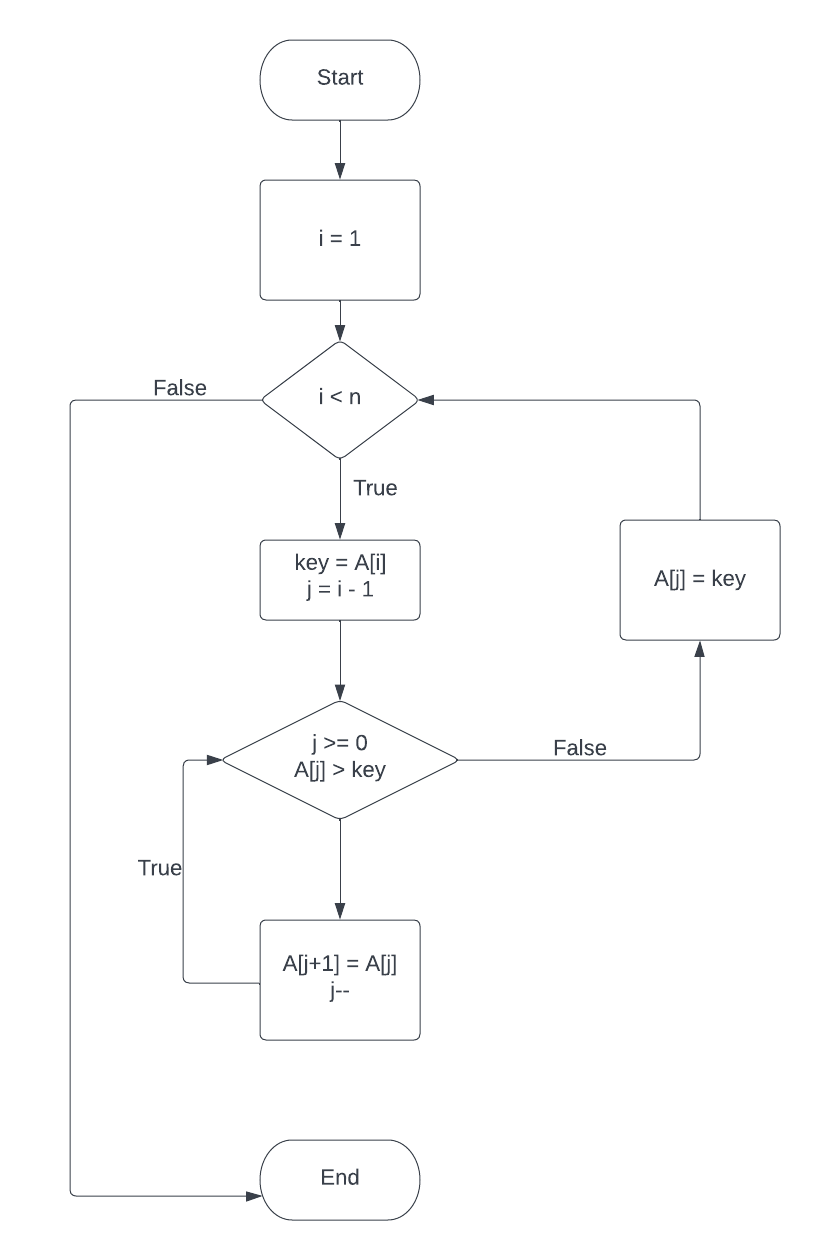
\includegraphics[width=0.6\textwidth]{Insertion Sort}
					\end{figure}
					
				\item \textbf{Description:}
					To sort an array of size N in ascending order: 
						\begin{itemize}
							\item Iterate from A[1] to A[N] over the array. 
							\item Compare the current element (x) to its predecessor. 
							\item If the key element is smaller than its predecessor, compare it to the elements before. Move the greater elements one position up to make space for the swapped element.
						\end{itemize}
				\item \textbf{Variants/ improvements:}
					\begin{itemize}
						\item Shell sort compares elements separated by a distance that decreases on each pass. Shell sort has distinctly improved running times in practical work, with two simple variants requiring $\mathcal{O}(n^{\sfrac{3}{2}})$ and $\mathcal{O}(n^{\sfrac{4}{3}})$ running time
						\item Binary insertion sort employs a binary search to determine the correct location to insert new elements, and therefore performs $\lceil log_{2}n \rceil$ comparisons in the worst case. When each element in the array is searched for and inserted this is $\mathcal{O}$(n log n). The algorithm as a whole still has a running time of $\mathcal{O}(n^2)$ on average because of the series of swaps required for each insertion
						that this sorting algorithm runs with high probability in $\mathcal{O}$(n log n) time.
						\item Binary merge sort uses a binary insertion sort to sort groups of 32 elements, followed by a final sort using merge sort. It combines the speed of insertion sort on small data sets with the speed of merge sort on large data sets.
						\item Library sort or gapped insertion sort that leaves a small number of unused spaces (i.e., "gaps") spread throughout the array. The benefit is that insertions need only shift elements over until a gap is reached. The authors show that this sorting algorithm runs with high probability in $\mathcal{O}$(n log n) time.
					\end{itemize}
				\item \textbf{Advantage, disadvantage:}
					\begin{table}[H]
						\centering
						\begin{tabular}{|p{8cm}|p{8cm}|}
							\hline
							\textbf{Advantage} & \textbf{Disadvantage} \\
							\hline
							\hline
							The main advantage of the insertion sort is its simplicity. 							 & The disadvantage of the insertion sort is that it does not perform as well as other, better sorting algorithms \\[12pt]
							It also exhibits a good performance when dealing with a small list. 					 & With n-squared steps required for every n element to be sorted, the insertion sort does not deal well with a huge list. \\[12pt]
							The insertion sort is an in-place sorting algorithm so the space requirement is minimal. & The insertion sort is particularly useful only when sorting a list of few items. \\
							\hline
						\end{tabular}
					\end{table}
				\item \textbf{Application:}	
					\begin{itemize}
						\item If the cost of comparisons exceeds the cost of swaps, as is the case for example with string keys stored by reference or with human interaction, then using binary insertion sort may yield better performance.
						\item A variant named binary merge sort uses a binary insertion sort to sort groups of 32 elements, followed by a final sort using merge sort.
						\item If a skip list is used, the insertion time is brought down to $\mathcal{O}$(log n), and swaps are not needed because the skip list is implemented on a linked list structure. The final running time for insertion would be $\mathcal{O}$(n log n).
					\end{itemize}
			\end{enumerate}
		
		\rule{15cm}{0.1cm}
		\subsection{Bubble Sort}
		\rule{15cm}{0.1cm}
			\begin{enumerate}[label=\textbf{\arabic*})]
				\item \textbf{Main idea:}
				Bubble Sort works by repeatedly swapping the adjacent elements if they are in the wrong order.
				\\[12pt]
				\item \textbf{Complexity Analysis of Bubble Sort}
				\begin{itemize}
							\item Bubble Sort is an in-place algorithm as it does not use any additional memory. Its algorithm is also stable.
							\item Bubble Sort has a huge number of swaps.
							\item The worst case condition for bubble sort occurs when elements of the array are arranged in decreasing order.
							\item Worst and average case time complexity is the same: $\mathcal{O}(n^2)$
							\item The best case occurs when an array is already sorted with time complexity: $\mathcal{O}(n)$
				\end{itemize}
				\item \textbf{Pseudo code:} 
			    \begin{algorithm}
            	\begin{algorithmic}[1]
            		\Procedure{Bubble Sort}{$a, n$}
            			\For {$i = 0 \textbf{ to }n-i-1$}
            				\For {$j = 0 \textbf{ to }n-i-2$}
            					\If{$a[j]>a[j+1]$}
            						\State Swap(a[j], a[j+1])
            					\EndIf
            				\EndFor
            			\EndFor
            		\EndProcedure
            	\end{algorithmic}
                \end{algorithm}
				\item \textbf{Flowchart:}
					\begin{figure}[H]
						\centering 
						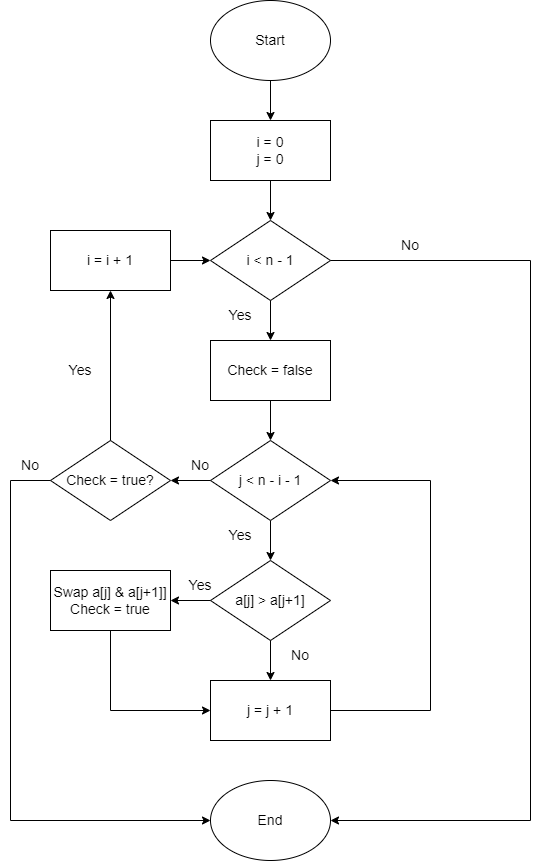
\includegraphics[width=0.6\textwidth]{BubbleSortFlowchart}
					\end{figure}
					
				\item \textbf{Description:}
						\begin{itemize}
							\item Step 1: assign $i = 0$
                            \item Step 2: assign $j = 0$, swapped = false
                            \item Step 3: if $a[j] > a[j+1]$, swap a[j] and a[j+1], swapped = true
                            \item Step 4: $j = j + 1$, if $j < n – i – 1$ go to step 3
                            \item Step 5: if swapped = false, end algorithm
                            \item Step 6: $i = i + 1$, if $i < n – 1$ go to step 2
						\end{itemize}
				\item \textbf{Variants/ improvements:}
					\begin{itemize}
						\item Odd–even sort is a parallel version of bubble sort, for message passing systems.
						\item Cocktail shaker sort alternates leftwards and rightwards passes.
					\end{itemize}
				\item \textbf{Advantage, disadvantage:}
					\begin{table}[H]
						\centering
						\begin{tabular}{|p{8cm}|p{8cm}|}
							\hline
							\textbf{Advantage} & \textbf{Disadvantage} \\
							\hline
							\hline
							Easy to understand, easy to implement & It takes a lot of time to sort \\[12pt]
							& It swaps too many times so it’s not efficient when swapping is costly\\
							\hline
						\end{tabular}
					\end{table}
				\item \textbf{Application:}	
					\begin{itemize}
						\item Due to its simplicity, bubble sort is often used to introduce the concept of a sorting algorithm.
						\item In computer graphics bubble sort is popular for its capability to detect a very small error (like swap of just two elements) in almost-sorted arrays and fix it with just linear complexity (2n).
					\end{itemize}
			\end{enumerate}
		
		\rule{15cm}{0.1cm}
		\subsection{Shaker Sort}
		\rule{15cm}{0.1cm}
			\begin{enumerate}[label=\textbf{\arabic*})]
				\item \textbf{Main idea:}
				Shaker Sort or Cocktail Sort is a variation of Bubble sort. The Bubble sort algorithm always traverses elements from left and moves the largest element to its correct position in first iteration and second largest in second iteration and so on. Cocktail Sort traverses through a given array in both directions alternatively. 
				\\[12pt]
				\item \textbf{Complexity Analysis of Shaker Sort}
				\begin{itemize}
				    \item Worst and Average Case Time Complexity: O($n^2$). 
                    \item Best Case Time Complexity: O(n). Best case occurs when array is already sorted.
				\end{itemize}   
				\item \textbf{Pseudo code:} 
				\begin{algorithm}[H]
            	\begin{algorithmic}[1]
            		\Procedure{Shaker Sort}{$a, n$}
            			\Do
            				\State $swapped \gets false$
            				\For{$i=0\textbf{ to }n-2$}
            					\State \textcolor{gray}{// test whether the two elements are in the wrong order}
            					\If{$a[i]>a[i+1]$}
            						\State \textcolor{gray}{// // let the two elements change places}
            						\State swap(a[i], a[i+1])
            						\State $swapped \gets true$
            					\EndIf
            				\EndFor
            				\If	{not swapped}
            					\State \textcolor{Gray}{// we can exit the outer loop here if no swaps occurred.}
            					\State break do-while loop
            				\EndIf
            				\State $swapped \gets false$
            				\For{$i=n-2\textbf{ to }0$}
            					 \If{$a[i]>a[i+1]$}
            						\State swap(a[i], a[i+1])
            						\State $swapped \gets true$
            					\EndIf
            				\EndFor
            			\doWhile{swapped} \Comment{\textcolor{Gray}{// if no elements have been swapped, then the list is sorted}}
            		\EndProcedure
            	\end{algorithmic}
            \end{algorithm}
				\item \textbf{Flowchart:}
					\begin{figure}[H]
						\centering 
						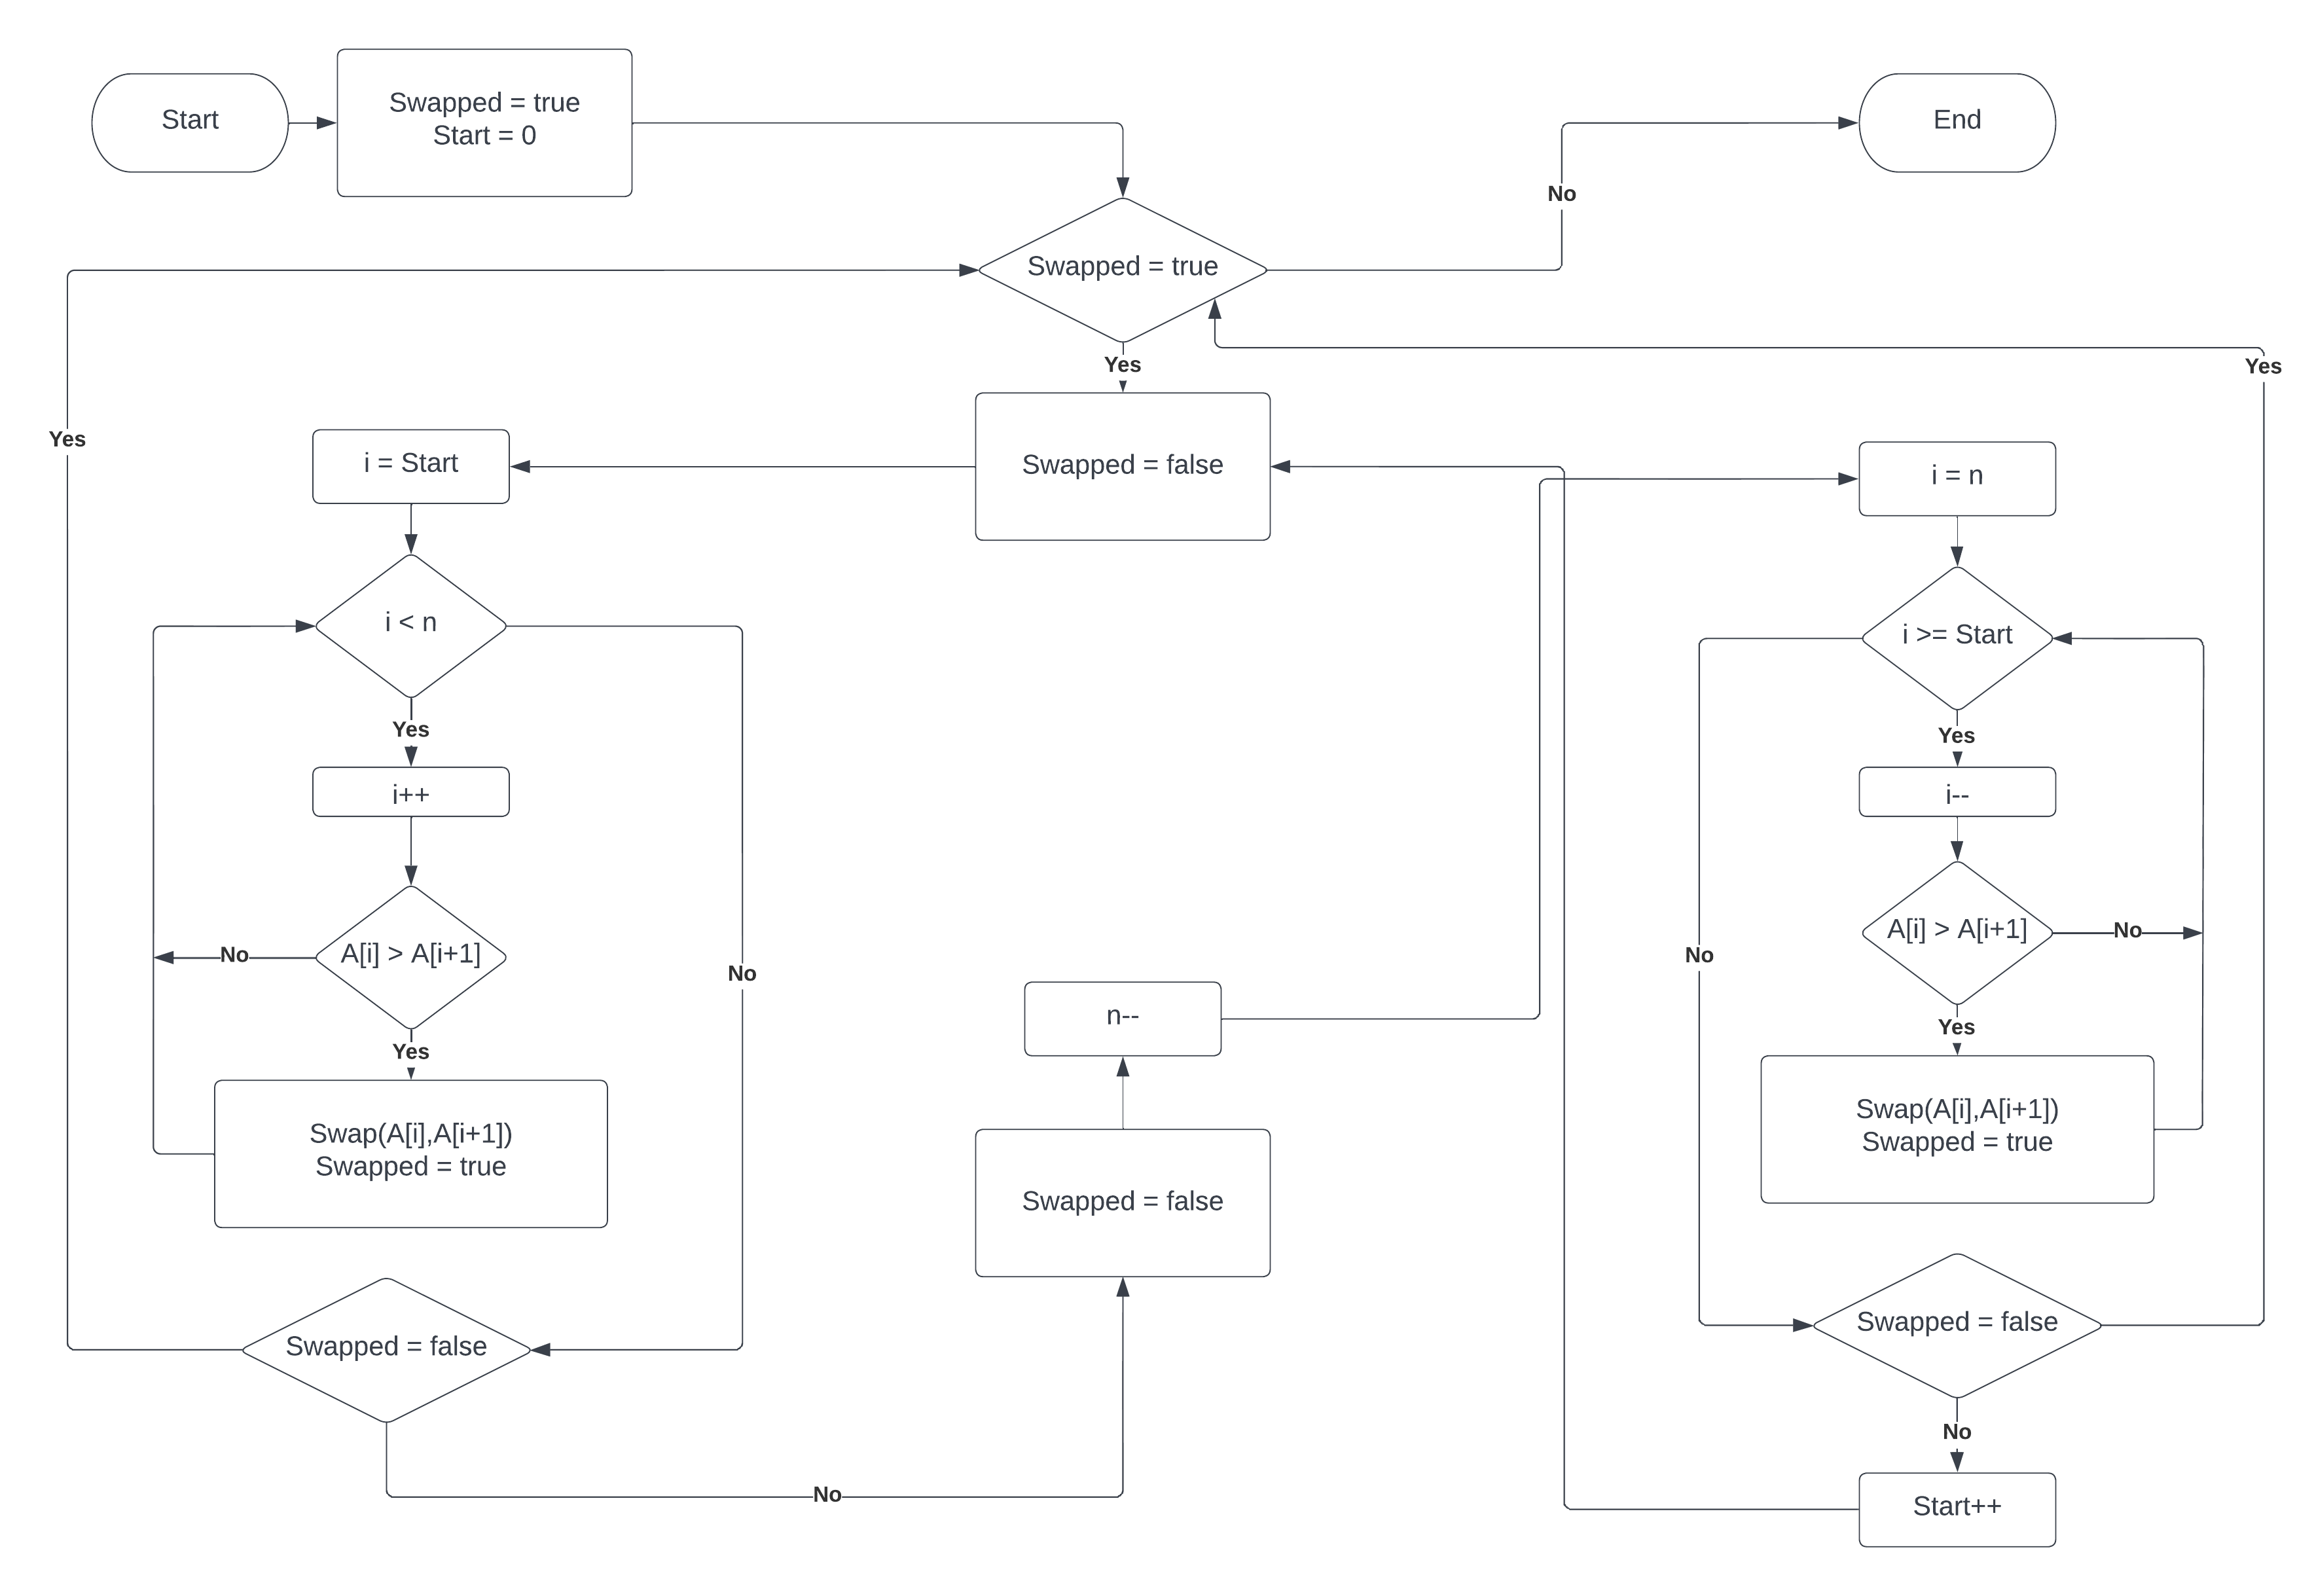
\includegraphics[width=0.8\textwidth]{Shaker Sort}
					\end{figure}
					
				\item \textbf{Description:}
					Each iteration of the algorithm is broken up into 2 stages: 
					\begin{itemize}
						\item The first stage loops through the array from left to right, just like the Bubble Sort. During the loop, adjacent items are compared and if value on the left is greater than the value on the right, then values are swapped. At the end of first iteration, largest number will reside at the end of the array.
						\item The second stage loops through the array in opposite direction- starting from the item just before the most recently sorted item, and moving back to the start of the array. Here also, adjacent items are compared and are swapped if required.
					\end{itemize}
				\item \textbf{Variants/ improvements:}
					\begin{itemize}
					\item Cocktail shaker sort, also known as bidirectional bubble sort, cocktail sort, shaker sort (which can also refer to a variant of selection sort), ripple sort, shuffle sort, or shuttle sort, is an extension of bubble sort. The algorithm extends bubble sort by operating in two directions. While it improves on bubble sort by more quickly moving items to the beginning of the list, it provides only marginal performance improvements.
                    
                    \item Like most variants of bubble sort, cocktail shaker sort is used primarily as an educational tool. More performant algorithms such as timsort, or merge sort are used by the sorting libraries built into popular programming languages such as Python and Java.
                    \end{itemize}
				\item \textbf{Advantage, disadvantage:}
					\begin{table}[H]
						\centering
						\begin{tabular}{|p{8cm}|p{8cm}|}
							\hline
							\textbf{Advantage} & \textbf{Disadvantage} \\
							\hline
							\hline
							The primary advantage of the shaker sort is that it a improvement of bubble sort and easy to implement & The main disadvantage of the shaker sort like bubble sort is the fact that it does not deal well with a list containing a huge number of items. \\[12pt]
							In the shaker sort, elements are swapped in place without using additional temporary storage. 		   & The shaker is mostly suitable for academic teaching but not for real-life applications.\\[12pt]
							The space requirement is at a minimum & \\[12pt]
							Easily get the largest and smallest element after first loop & \\
							\hline
						\end{tabular}
					\end{table}
				\item \textbf{Application:}	
					\begin{itemize}
						\item An example of a list that proves this point is the list (2,3,4,5,1), which would only need to go through one pass of cocktail sort to become sorted, but if using an ascending bubble sort would take four passes. However one Shaker Sort pass should be counted as two Bubble Sort passes. Typically Shaker Sort is less than two times faster than Bubble Sort.
						\item Another optimization can be that the algorithm remembers where the last actual swap has been done. In the next iteration, there will be no swaps beyond this limit and the algorithm has shorter passes. As the Shaker Sort goes bidirectionally, the range of possible swaps, which is the range to be tested, will reduce per pass, thus reducing the overall running time slightly. So in some occasion we can use Shaker Sort rather than Bubble Sort to reduce time and resouce consuming
					\end{itemize}
			\end{enumerate}
		
		\rule{15cm}{0.1cm}
		\subsection{Shell Sort}
		\rule{15cm}{0.1cm}
			\begin{enumerate}[label=\textbf{\arabic*})]
				\item \textbf{Main idea:}
				Method of Shell Sport starts by sorting pairs of elements far apart from each other, then progressively reducing the gap between elements to be compared.
				\\[12pt]
				\item \textbf{Complexity Analysis of Shell Sort}
				\begin{itemize}
				\item Shell Sort is an optimization of insertion sort that allows the exchange of items that are far apart.
                \item By starting with far apart elements, it can move some out-of-place elements into position faster than a simple nearest neighbor exchange
                \item Shell Sort is an in-place sorting algorithm, but it’s not stable
                \item The worst case time complexity for shell sort is O($n^2$)
                \item When the given array list is already sorted the total count of comparisons of each interval is equal to the size of the given array. So best case time complexity is O(nlog(n))
                \item The shell sort average case time complexity depends on the interval selected by the programmer.
                \item The space complexity of the shell sort is O(1)
                \end{itemize}
				\item \textbf{Pseudo code:} 
				\begin{algorithm}[H]
            	\begin{algorithmic}[1]
            		\Procedure{Shell Sort}{$a, n$}
            			\State \textcolor{Gray}{/* calculate interval*/}
            			\While{$interval < n/3$}
            				\State $interval = interval*3+1$ 
            			\EndWhile
            			\While{$interval > 0$}
            				\For {$outer=interval\textbf{ to }n$}
            					\State \textcolor{Gray}{/* select value to be inserted */}
            					\State $valueToInsert = a[outer]$
            					\State $inner = outer$
            					\State \textcolor{Gray}{/*shift element towards right*/}
            					\vspace{12pt}
            					\While{$inner > interval - 1 \textbf{ and } a[inner - interval] \geq valueToInsert$}
            						\State $a[inner] = a[inner-interval]$
            						\State $inner = inner - interval$
            					\EndWhile
            					\vspace{12pt}
            					\State \textcolor{Gray}{/* insert the number at hole position */}
            					\State $a[inner] = valueToInsert$
            				\EndFor
            				\State \textcolor{Gray}{/* calculate interval*/}
            				\State $interval = (interval-1)/3$
            			\EndWhile
            		\EndProcedure
            	\end{algorithmic}
            \end{algorithm}
				\item \textbf{Flowchart:}
					\begin{figure}[H]
						\centering 
						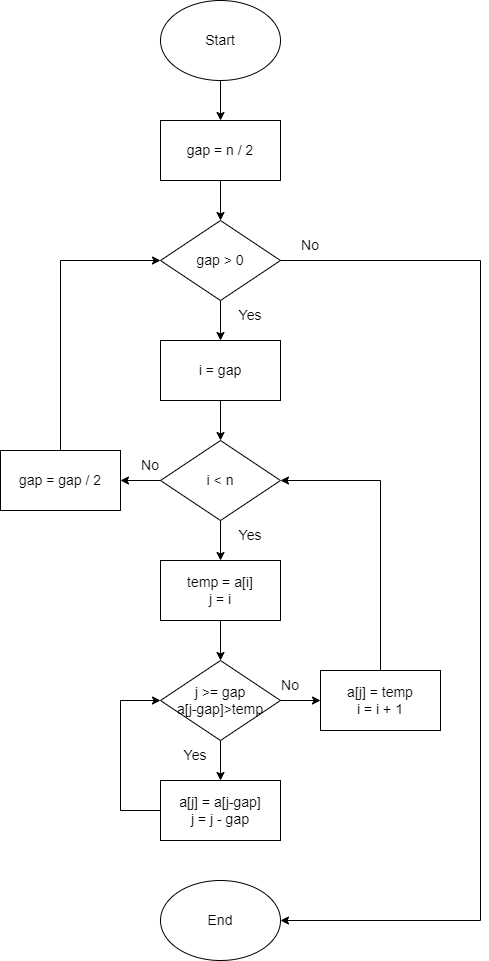
\includegraphics[width=0.5\textwidth]{ShellSortFlowchart}
					\end{figure}
					
				\item \textbf{Description:}
					\begin{itemize}
						\item Step 1: Initialize the value of gap size. Example: h
                        \item Step 2: Divide the list into smaller sub-part. Each must have equal intervals to h
                        \item Step 3: Sort these sub-lists using insertion sort
                        \item Step 4: Repeat step 2 until the list is sorted
					\end{itemize}
				\item \textbf{Variants/ improvements:}
					Shell sort is mainly a variation of Insertion Sort. In insertion sort, we move elements only one position ahead. When an element has to be moved far ahead, many movements are involved. The idea of ShellSort is to allow the exchange of far items. In Shell sort, we make the array h-sorted for a large value of h. We keep reducing the value of h until it becomes 1. An array is said to be h-sorted if all sublists of every h’th element are sorted.
				\item \textbf{Advantage, disadvantage:}
					\begin{table}[H]
						\centering
						\begin{tabular}{|p{8cm}|p{8cm}|}
							\hline
							\textbf{Advantage} & \textbf{Disadvantage} \\
							\hline
							\hline
							Shell Sort is more efficient for medium size arrays than Insertion Sort and Bubble Sort & It is a complex algorithm \\[12pt]
							It’s space complexity is O(1)  & It is not as efficient as merge sort and quick sort\\[12pt]
							 & It is unstable\\
							\hline
						\end{tabular}
					\end{table}
				\item \textbf{Application:}	
					\begin{itemize}
						\item Shell Sort performs more operations and has higher cache miss ratio than quicksort
						\item Shell Sort can also serve as a sub-algorithm of introspective sort, to sort short subarrays and to prevent a slowdown when the recursion depth exceeds a given limit
					\end{itemize}
			\end{enumerate}
		
		\rule{15cm}{0.1cm}
		\subsection{Heap Sort}
		\rule{15cm}{0.1cm}
			\begin{enumerate}[label=\textbf{\arabic*})]
				\item \textbf{Main idea:}
				
					Heapsort can be considered an improvement of selection sort. However, the difference is heap sort is performed on the heap data structure. Heap is a complete binary tree. Heap tree can be of two types. Min-heap or max-heap. For min heap the root element is minimum and for max heap the root is maximum. After forming a heap, we can delete an element from the root and send the last element to the root. After these swapping procedures, we need to re-heap the whole array. By deleting elements from root we can sort the whole array.
				\\[12pt]
				\item \textbf{Complexity Analysis of Heap Sort}
					
					Let’s say n is the number of elements in the array. 
					\\[9pt]
					\textbf{Time complexity:}
					
					Heapsort’s complexity can be calculated through 2 main processes: making an array heapified and and and getting a sorted array from a heapified one.
					By some mathematical properties, we can say building a heap out of a randomly arranged array, can be done in O(n).
					About getting a sorted array out of a max heap,this step involves swapping the leftmost value in the array with the rightmost value in the array occupied by the heap and reheapification of the new smaller heap. Swapping the max element with the bottom level rightmost element and reducing the size of the heap can be done in constant time, O(1). Now, let’s discuss reheapification. In the worst case, the new value at the root position will have to be swapped log(N) times to be sent to the bottom of the heap to achieve a MaxHeap once again. So each reheapification after the extraction costs O(logn).
					The total time complexity of heap sort can be calculated as the total of 2 above steps, which equals to O(n log(n))
					\\[9pt]
					\textbf{Space complexity:}
					
					Heapsort is an in-place sorting method, i.e., no additional memory space is required except for loop and auxiliary variables. The number of these variables is always the same. Therefore the space complexity of heapsort is O(1).
				\\[12pt]
				\item \textbf{Pseudo code:} 
				\begin{algorithm}[H]
            	\begin{algorithmic}[1]
            		\Procedure{Heapify}{a, n, i}
            			\State $max \gets i$
            			\State $leftchild \gets 2i+1$
            			\State $rightchild \gets 2i+2$
            			\If{$leftchild \leq n \textbf{ and } a[i] < a[leftchild]$}
            				\State $max \gets leftchild$
            			\Else
            				\State $max \gets i$
            			\EndIf
            			\If{$rightchild \leq n \textbf{ and } a[max] > a[rightchild]$}
            				\State $max \gets rightchild$
            			\EndIf
            			\If{$max \neq i$}
            				\State Swap(a[i], a[max])
            				\State Heapify(a, n, max)
            			\EndIf
            		\EndProcedure
            		\vspace{12pt}
            		\Procedure{Heap Sort}{$a \text{: array, } n \text{: number of elements}$}
            			\For {$i=n/2 \textbf{ downto }1$}
            				Heapify(a, n, i)
            			\EndFor
            			
            			\For{$i=n \textbf{ downto } 2$}
            				\State Exchange a[1] with a[i]
            				\State $n \gets n - 1$
            				\State Heapify(a, i, 0)
            			\EndFor
            		\EndProcedure
            	\end{algorithmic}
            \end{algorithm}
				\item \textbf{Flowchart:}
					\begin{figure}[H]
						\centering 
						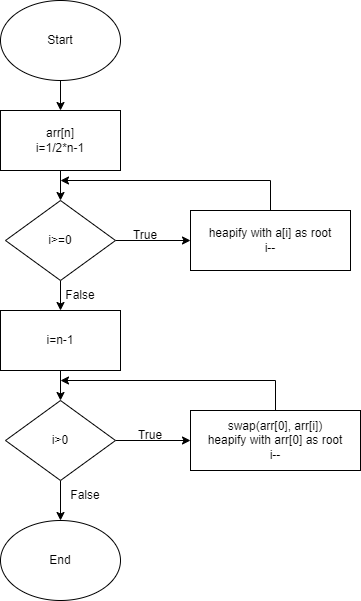
\includegraphics[width=0.5\textwidth]{HeapSort Flowchart}
					\end{figure}
					
				\item \textbf{Description:}
					\begin{enumerate}
						\item We start by using Heapify to build a max heap of elements present in an array A.
						\item Once the heap is ready, the largest element will be present in the root node of the heap that is A[0].
						\item Now swap the element at A[0] with the last element of the array, and heapify the max heap excluding the last element.
						\item Repeat steps b and c till all the elements in the array are sorted.
					\end{enumerate}
				\item \textbf{Variants/ improvements:}
				
					\textbf{Ternary heapsort}
					
					Ternary heapsort uses a ternary heap instead of a binary heap; that is, each element in the heap has three children. It is more complicated to program, but does a constant number of times fewer swap and comparison operations. This is because each step in the shift operation of a ternary heap requires three comparisons and one swap, whereas in a binary heap two comparisons and one swap are required. The ternary heap does two steps in less time than the binary heap requires for three steps, which multiplies the index by a factor of 9 instead of the factor 8 of three binary steps. Ternary heapsort is about 12% faster than the simple variant of binary heapsort.
					\\[9pt]
					\textbf{Smoothsort}
					
					The smoothsort algorithm is a variation of heapsort developed by Edsger Dijkstra in 1981. Like heapsort, smoothsort's upper bound is O(n log n). The advantage of smoothsort is that it comes closer to O(n) time if the input is already sorted to some degree, whereas heapsort averages O(n log n) regardless of the initial sorted state. Due to its complexity, smoothsort is rarely used.
					\\[9pt]
					\textbf{Heapsort based on a Cartesian tree}
					
					Levcopoulos and Petersson describe a variation of heapsort based on a Cartesian tree that does not add an element to the heap until smaller values on both sides of it have already been included in the sorted output. As they show, this modification can allow the algorithm to sort more quickly than O(n log n) for inputs that are already nearly sorted.
				\item \textbf{Advantage, disadvantage:}
					\begin{table}[H]
						\centering
						\begin{tabular}{|p{8cm}|p{8cm}|}
							\hline
							\textbf{Advantage} & \textbf{Disadvantage} \\
							\hline
							\hline
							Performance is optimal. This implies that no other sorting algorithms can perform better in comparison. & Maintaining a heap is not easy. \\[12pt]
							Memory usage is minimal because apart from what is necessary to hold the initial list of items to be sorted, it needs no additional memory space to work. & Heapsort is unstable sort. It might rearrange the relative order.\\[12pt]
							The Heap sort algorithm exhibits consistent performance. This means it performs equally well in the best, average and worst cases. Because of its guaranteed performance, it is particularly suitable to use in systems with critical response time. & Heapsort cannot be used when dataset is really huge and doesn't fit into memory\\
							\hline
						\end{tabular}
					\end{table}
				\item \textbf{Application:}	
					\begin{itemize}
						\item Implementation of priority queues
						\item Security systems
						\item Embedded systems (for example, Linux Kernel)
					\end{itemize}
			\end{enumerate}
		
		\rule{15cm}{0.1cm}
		\subsection{Merge Sort}
		\rule{15cm}{0.1cm}
			\begin{enumerate}[label=\textbf{\arabic*})]
				\item \textbf{Main idea:}
				
					Merge Sort is a Divide and Conquer algorithm. It divides the input array into two halves, calls itself for the two halves, and then it merges the two sorted halves. The merge() function is used for merging two halves. The merge(arr, l, m, r) is a key process that assumes that arr[l..m] and arr[m+1..r] are sorted and merges the two sorted sub-arrays into one
				\\[12pt]
				\item \textbf{Complexity Analysis of Merge Sort}
    				
    				Time complexity of Merge Sort is O(n*Log n) in all the 3 cases (worst, average and best) as merge sort always divides the array in two halves and takes linear time to merge two halves.
				\\[12pt]
				\item \textbf{Pseudo code:} 
				\begin{algorithm}
            	\begin{algorithmic}[1]
            		\Procedure{Merge Sort}{$a, n$}
            			\If{$n == 1$} 
            				\State return a
            			\EndIf
            			\State l1 as array = a[0]...a[$n/2$]
            			\State l2 as array = a[$n/2+1$]...a[n]
            			\State l1 = mergeSort(l1)
            			\State l2 = mergeSort(l2)
            			\State return merge(l1, l2)
            		\EndProcedure
            		\vspace{12pt}
            		\Procedure{merge}{a: array, b: array}
            			\State c as array
            			\While {a and b have elements}
            				\If{$a[0]>b[0]$}
            					\State add b[0] to the end of c
            					\State remove b[0] from b
            				\Else 
            					\State add a[0] to the end of c
            					\State remove a[0] from a
            				\EndIf
            			\EndWhile
            			\While {a has elements}
            				\State add a[0] to the end of c
            				\State remove a[0] from a
            			\EndWhile
            			\While {b has elements}
            				\State add b[0] to the end of c
            				\State remove b[0] from a
            			\EndWhile
            			
            			\State return c
            		\EndProcedure
            	\end{algorithmic}
            \end{algorithm}
				\item \textbf{Flowchart:}
					\begin{figure}[H]
						\centering 
						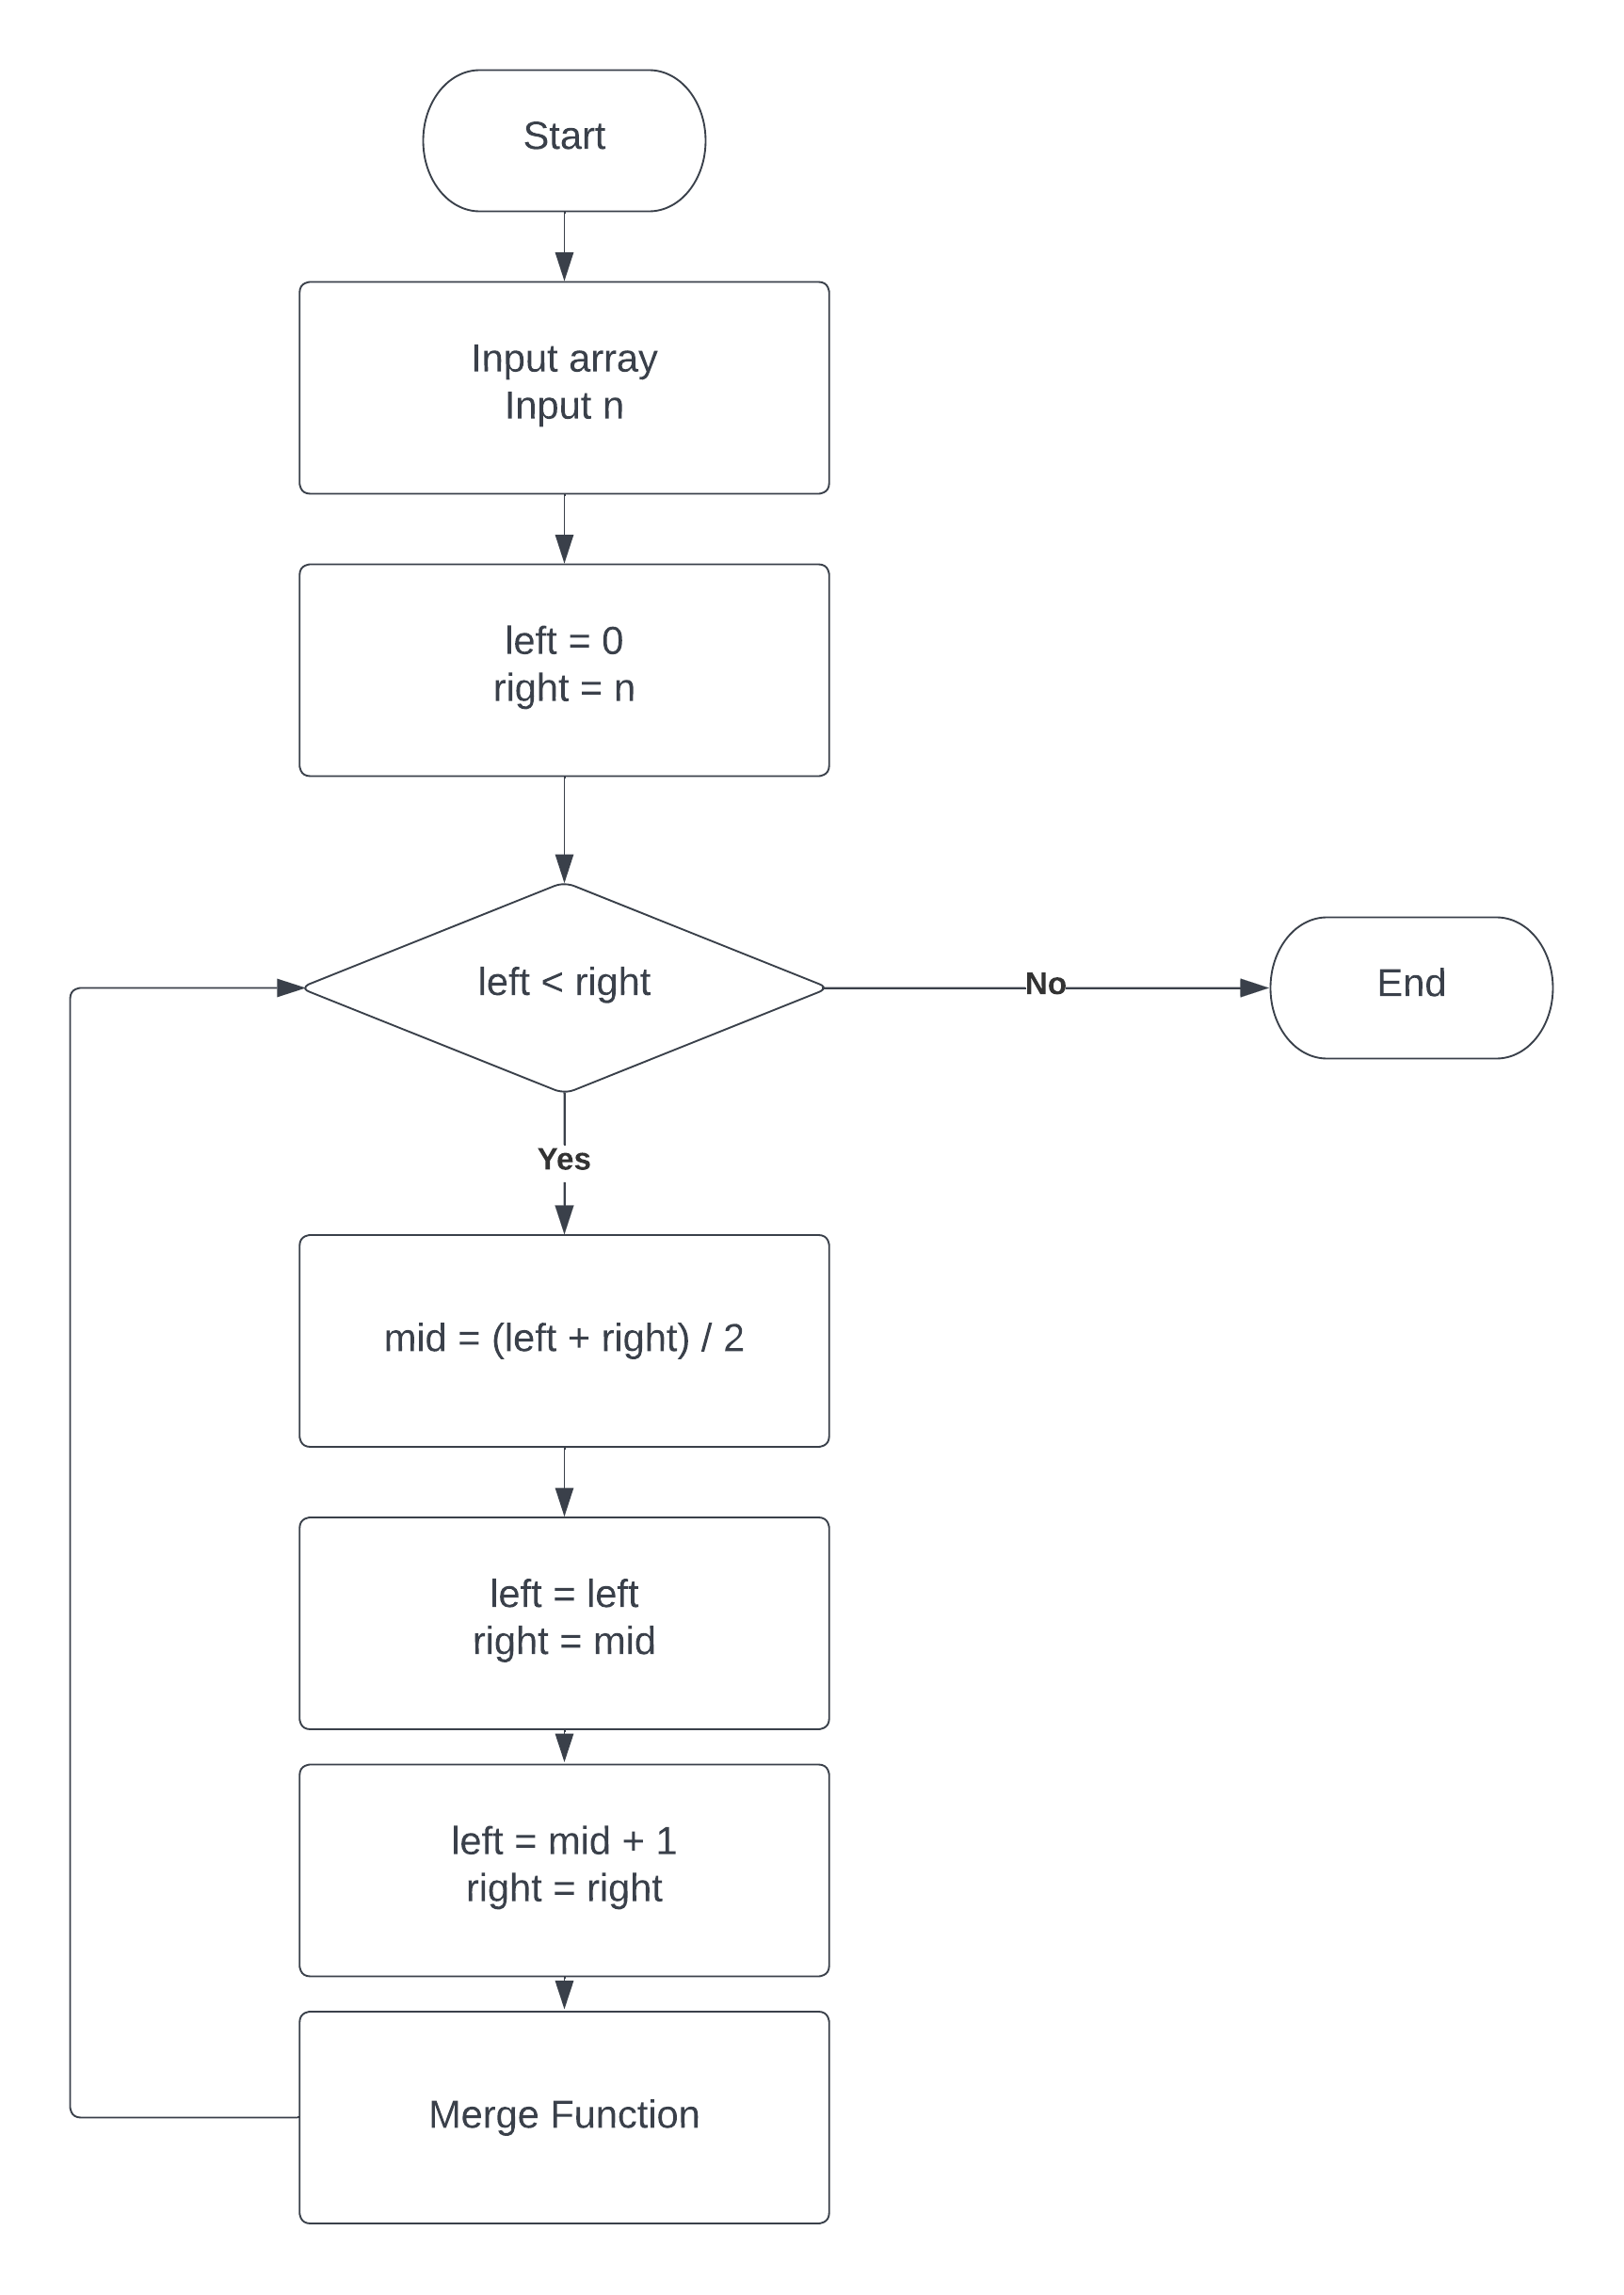
\includegraphics[width=0.5\textwidth]{Merge Sort}
					\end{figure}
					
				\item \textbf{Description:}
					Declare left variable to 0 and right variable to n-1 
					\begin{itemize}
						\item Find mid by medium formula. mid = (left+right)/2
						\item Call merge sort on (left,mid)
						\item Call merge sort on (mid+1,rear)
						\item Continue till left is less than right
						\item Then call merge function to perform merge sort.
					\end{itemize}
				\item \textbf{Variants/ improvements:}
					\begin{itemize}
						\item 3-way merge sort where instead of splitting the array into 2 parts we split it into 3 parts. Merge sort recursively breaks down the arrays to subarrays of size half. Similarly, 3-way Merge sort breaks down the arrays to subarrays of size one third. 
						\item binary merge sort uses a binary insertion sort to sort groups of 32 elements, followed by a final sort using merge sort. It combines the speed of insertion sort on small data sets with the speed of merge sort on large data sets.
					\end{itemize}
				\item \textbf{Advantage, disadvantage:}
					\begin{table}[H]
						\centering
						\begin{tabular}{|p{8cm}|p{8cm}|}
							\hline
							\textbf{Advantage} & \textbf{Disadvantage} \\
							\hline
							\hline
							It can be applied to files of any size. & Requires extra space »N \\[12pt]
							Reading of the input during the run-creation step is sequential $\rightarrow$ Not much seeking. & Merge Sort requires more space than other sort.\\[12pt]
							If heap sort is used for the in-memory part of the merge, its operation can be overlapped with I/O & Merge sort is less efficient than other sort\\
							\hline
						\end{tabular}
					\end{table}
				\item \textbf{Application:}	
					\begin{itemize}
						\item Merge Sort is useful for sorting linked lists in O(nLogn) time. In the case of linked lists, the case is different mainly due to the difference in memory allocation of arrays and linked lists. Unlike arrays, linked list nodes may not be adjacent in memory. Unlike an array, in the linked list, we can insert items in the middle in O(1) extra space and O(1) time. Therefore, the merge operation of merge sort can be implemented without extra space for linked lists.
						\item In arrays, we can do random access as elements are contiguous in memory. Let us say we have an integer (4-byte) array A and let the address of A[0] be x then to access A[i], we can directly access the memory at (x + i*4). Unlike arrays, we can not do random access in the linked list. Quick Sort requires a lot of this kind of access. In a linked list to access i’th index, we have to travel each and every node from the head to i’th node as we don’t have a continuous block of memory. Therefore, the overhead increases for quicksort. Merge sort accesses data sequentially and the need of random access is low.
						\item Inversion Count Problem
						\item Used in External Sorting
					\end{itemize}
			\end{enumerate}
		
		\rule{15cm}{0.1cm}
		\subsection{Quick Sort}
		\rule{15cm}{0.1cm}
			\begin{enumerate}[label=\textbf{\arabic*})]
				\item \textbf{Main idea:}
				
					Quick Sort picks an element as pivot and partitions the given array around the picked pivot. Then, it sorts the parts independently. Finally, it combines the sorted subsequences by a simple concatenation.
				\\[12pt]
				\item \textbf{Complexity Analysis of Quick Sort}
					\begin{itemize}
					\item Quick Sort is based on the divide-and-conquer paradigm
                    \item Quick Sort is an in-place sorting algorithm, it just requires small additional amounts of memory to perform the sorting. However, Quick Sort is not stable
                    \item It’s efficiency based on which elements we chose as pivot
                    \item Worst case occurs if the pivot happens to be the smallest or largest element in the list, or in some implementations all the elements are equal. If this happens repeatedly in every partition, then each recursive call processes a list of size one less than the previous list. In this case Quick Sort takes O($n^2$) time
                    \item Best case occurs if each time we perform a partition we divide the list into two nearly equal pieces. This means each recursive call processes a list of half the size. Quick Sort takes only O(nlog(n)) time in this case
                    \item Average case, Quick Sort takes O(nlog(n)) time
                    \item The space used by quicksort depends on the version used. The in-place version of quicksort has a space complexity of O(log(n)), even in the worst case, when it is carefully implemented
                    \end{itemize}
				\item \textbf{Pseudo code:} 
				\begin{algorithm}[H]
            	\begin{algorithmic}[1]
            		\Procedure{Quick Sort}{a, begin, end}
            			\State pivotIndex = partition(a, begin, end)
            			\State quickSort(a, begin, pivotIndex)
            			\State quickSort(a, pivotIndex + 1, end)
            		\EndProcedure
            		
            		\Procedure{Partition}{a, begin, end}
            			\State set end as pivotIndex
            			\State pIndex = beg - 1
            			\For{$i=beg\textbf{ to }end-1$}
            				\If{$a[i] < pivot$}
            					\State Swap a[i] and a[pIndex]
            					\State pIndex++
            				\EndIf
            			\EndFor
            			\State Swap pivot and a[pIndex + 1]
            			\State return pIndex + 1
            		\EndProcedure
            	\end{algorithmic}
            \end{algorithm}
				\item \textbf{Flowchart:}
					\begin{figure}[H]
						\centering 
						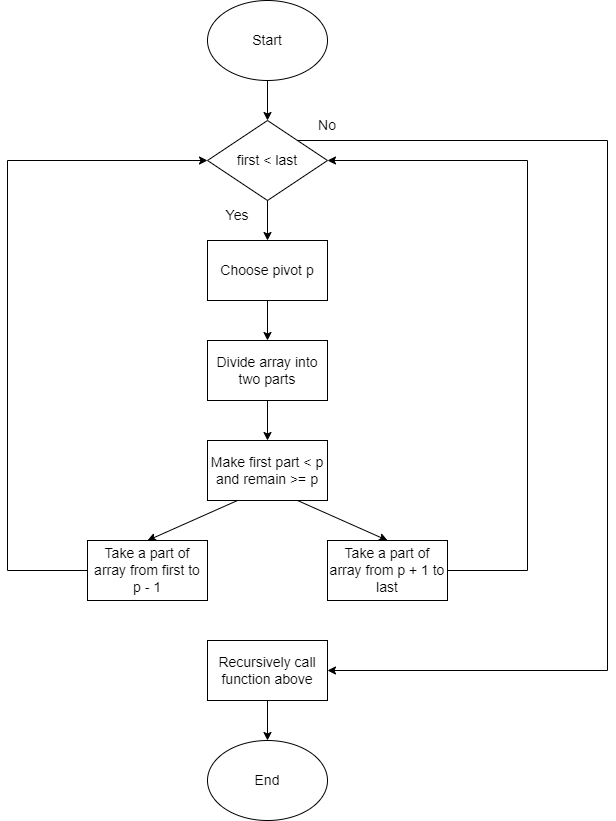
\includegraphics[width=0.5\textwidth]{QuickSortFlowChart}
					\end{figure}
					
				\item \textbf{Description:}
				\begin{itemize}
					\item Step 1: Choose pivot
                    \item Step 2: Divide the list into two parts
                    \item Step 3: Partition the elements so that all those with values less than the pivot come in one sub-list and all those with greater values come in another
                    \item Step 4: Run from step 1 with two sub-lists separately	
				\end{itemize}
				\item \textbf{Variants/ improvements:}
					\begin{itemize}
						\item Multi-pivot quicksort: Instead of partitioning into two subarrays using a single pivot, multi-pivot quicksort (also multiquicksort[25]) partitions its input into some s number of subarrays using s - 1 pivots. The performance benefit of this algorithm was subsequently found to be mostly related to cache performance,[36] and experimental results indicate that the three-pivot variant may perform even better on modern machines.
                        \item External quicksort: For disk files, an external sort based on partitioning similar to quicksort is possible. It is slower than external merge sort, but doesn't require extra disk space.
						\item Quick radix sort: This is again a combination of radix sort and quicksort but quick radix sort will avoid the worst case O($N^2$) behaviours of standard quicksort and radix quicksort, and will be faster even in the best case of those comparison algorithms
                        \item Three-way radix quicksort: This algorithm is a combination of radix sort and quicksort.
                        \item BlockQuicksort: BlockQuicksort rearranges the computations of quicksort to convert unpredictable branches to data dependencies.
					\end{itemize}
				\item \textbf{Advantage, disadvantage:}
					\begin{table}[H]
						\centering
						\begin{tabular}{|p{8cm}|p{8cm}|}
							\hline
							\textbf{Advantage} & \textbf{Disadvantage} \\
							\hline
							\hline
							Its running time is fast as it time complexity is O(nlog(n)) & In the worst case its time complexity is $O(n^2)$ \\[12pt]
							It is an in-place sorting algorithm & It is unstable\\[12pt]
							When implemented well, it can be somewhat faster than merge sort and about two or three times faster than heapsort & It is recursive so it may suffer stack overflow when the data’s size is big\\
							\hline
						\end{tabular}
					\end{table}
				\item \textbf{Application:}	
					\begin{itemize}
						\item Commercial Computing is used in various government and private organizations for the purpose of sorting various data
						\item The sorting algorithm is used for information searching and as Quicksort is one of the fastest algorithms so it is widely used as a better way of searching.
					\end{itemize}
			\end{enumerate}
			
		\rule{15cm}{0.1cm}
		\subsection{Counting Sort}
		\rule{15cm}{0.1cm}
			\begin{enumerate}[label=\textbf{\arabic*})]
				\item \textbf{Main idea:}
				
					Counting sort is an algorithm used to sort the elements of an array by counting and storing the frequency of each distinct element in an auxiliary array. Sorting is done by mapping the value of each element as an index of the auxiliary array.
				\\[12pt]
				\item \textbf{Complexity Analysis of Counting Sort}
					
					Let’s say n is the number of elements in the array, k is the range from the minimum value to the maximum value. 
					\\[9pt]
					\textbf{Time complexity:}
					
					Initializing the count array will take k seconds. k times to preserve the count array. Now you will do the actual sorting by iterating over the input array linearly.
					So that the time complexity of Counting sort is O(n+k).
					
					\textbf{Best case:} Occurs when all items are in the same range, or when k is equal to 1. In this scenario,  total time complexity is O(n), which is linear.
					
					\textbf{Worst case:} Occurs when the data range is huge, the maximum value is much bigger than the minimum one. In that case, the time complexity is O(n+k).
					
					\textbf{Average case:} To calculate the average case time complexity, fix N and take various values of k from 1 to infinity; in this scenario, k computes to (k+1/2), and the average case is N+(K+1)/2. However, because K approaches infinity, K is the essential element. Similarly, varying N reveals that both N and K are equally dominating, resulting in O(N+K) as the average case.
					
					\textbf{Space complexity}
					\\[9pt]
					Counting sort requires employing an auxiliary array of size k and an array to element in order which has n value. As a result, the Counting Sort algorithm has  space complexity O(n+k). The best case, worst case and average case are the same as time complexity
				\\[12pt]
				\item \textbf{Pseudo code:} 
				\begin{algorithm}
            	\begin{algorithmic}[1]
            		\Procedure{Counting Sort}{$a, n$}
            			\State\textcolor{Gray}{//a[]-- Initial Array to Sort}
            			\State\textcolor{Gray}{//Complexity: O(k)}
            			\For{$i=0\textbf{ to }k$}
            				\State c[i] = 0
            			\EndFor
            			\vspace{12pt}
            			\State\textcolor{Gray}{//Storing Count of each element}
            			\State\textcolor{Gray}{//Complexity: O(n)}
            			\For{$j=0\textbf{ to }n$}
            				\State c[a[j]] = c[a[j]] + 1
            			\EndFor
            			\vspace{12pt}
            			\State \textcolor{Gray}{//Change c[i] such that it contains actual}
            			\State \textcolor{Gray}{//position of these elements in output array}
            			\State \textcolor{Gray}{//Complexity: O(k)}
            			\For{$i=1\textbf{ to }k$}
            				\State c[i] = c[i] + c[i-1]
            			\EndFor
            			\vspace{12pt}
            			\State \textcolor{Gray}{//Build Output array from c[i]}
            			\State \textcolor{Gray}{//Complexity: O(n)}
            			\For{$j=n-1\textbf{ downto }0$}
            				\State  b[c[a[j]]-1] = a[j]
            				\State c[a[j]] = c[a[j]] - 1
            			\EndFor
            		\EndProcedure
            	\end{algorithmic}
            \end{algorithm}
				\item \textbf{Flowchart:}
					\begin{figure}[H]
						\centering 
						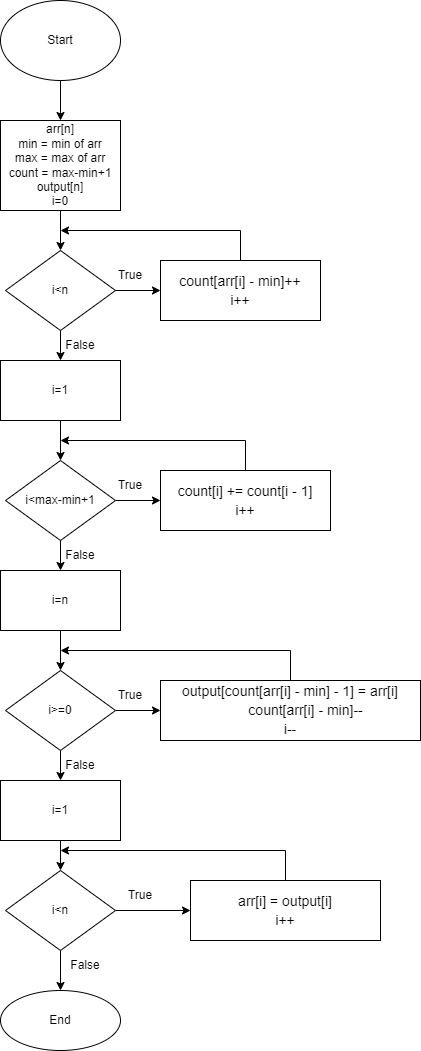
\includegraphics[width=0.5\textwidth]{CountingSort Flowchart}
					\end{figure}
					
				\item \textbf{Description:}
				\begin{itemize}
					\item 	Declare an auxiliary array Aux[] of size max(Arr[])+1 and initialize it with 0.
					\item Traverse array Arr[] and map each element of Arr[] as an index of Aux[] array, i.e., execute Aux[Arr[i]]++ for 0 <= i < N.  
					\item Calculate the prefix sum at every index of array Arr[]. 
					\item Create an array sortedArr[] of size N.
					\item Traverse array Arr[] from right to left and update sortedArr[] as sortedArr[ Aux[ Arr[i] ] - 1] - Arr[i]. Also, update Aux[] as  Aux[ Arr[i] ]--.
				\end{itemize}
				
				\item \textbf{Advantage, disadvantage:}
					\begin{table}[H]
						\centering
						\begin{tabular}{|p{8cm}|p{8cm}|}
							\hline
							\textbf{Advantage} & \textbf{Disadvantage} \\
							\hline
							\hline
							Counting sort generally performs faster than all comparison-based sorting algorithms, such as merge sort and quicksort, if the range of input is of the order of the number of input  & Counting sort doesn’t work on decimal values \\[12pt]
							Counting sort is easy to code & Counting sort is inefficient if the range of values to be sorted is very large \\
							\hline
						\end{tabular}
					\end{table}
				\item \textbf{Application:}	
					\begin{itemize}
						\item If the range of input data is not much bigger than the number of objects to be sorted, counting sort is efficient. Consider the following scenario: the data is 10, 5, 10K, 5K, and the input sequence is 1 to 10K
						\item It's frequently used as a subroutine in other sorting algorithms, such as radix sort.
						\item Counting sort counts the occurrences of the data object in O using partial hashing (1).
					\end{itemize}
			\end{enumerate}
			
		\rule{15cm}{0.1cm}
		\subsection{Radix Sort}
		\rule{15cm}{0.1cm}
			\begin{enumerate}[label=\textbf{\arabic*})]
				\item \textbf{Main idea:}
				
					Radix sort algorithm is a non-comparative sorting algorithm in computer science. It avoids comparison by creating and categorizing elements based on their radix. For elements with more than one significant digit, it repeats the bucketing process for each digit while preserving the previous step's ordering until all digits have been considered.
				\\[12pt]
				\item \textbf{Complexity Analysis of Radix Sort}
					
					Let’s say n is the number of elements in the array, p is the number of digits in the maximum number, d is the base of the number system used . 
					\\[9pt]
					\textbf{Time complexity:}
				
				Radix sort has the time complexity O(p*(n+d)).
				
				\textbf{Best case:} occurs when all elements have the same number of digits. O(p(n+d)) is the best-case time complexity. If d equals O(n), the time complexity is O. (p*n).
				
				\textbf{Worst case:} occurs when all elements have the same number of digits except one, which has a significantly large number of digits. If the number of digits in the largest element equals n, the runtime is $O(n^2)$.
				
				\textbf{Average case:} O(p*(n+d))
				\\[9pt]
					\textbf{Space complexity:}
				
				Because Radix sort employs Counting sort (in this report), which uses auxiliary arrays of sizes n and k, where n is the number of elements in the input array and k is the range from the maximum value in the array to the minimum value of the input array. Hence, the Radix sort has a space complexity of (n+k).
				\\[12pt]
				\item \textbf{Pseudo code:} 
				\begin{algorithm}
            	\begin{algorithmic}[1]
            		\Procedure{Radix Sort}{$a, d$}
            		\State \textcolor{Gray}{//It works same as counting sort for d number of passes}
            		\State \textcolor{Gray}{//Each key in a[0..n-1] is a d-digit integer}
            		\State \textcolor{Gray}{//Digits are numbered 1 to d from right to left}
            		\For {$j=1\textbf{ to }d$}
            			\State \textcolor{Gray}{//a[]-- Initial Array to sort}
            			\State int count[10] = \{0\}
            			\State \textcolor{Gray}{//Store the count of "keys" in count[]}
            			\State \textcolor{Gray}{//key- it is number at digit place j}
            			\For {$i=0\textbf{ to }n$}
            				\State count[key of (a[i]) in pass j]++
            			\EndFor
            			\For{$i=1\textbf{ to }10$}
            				\State count[k] = count[k] + count[k-1]
            			\EndFor
            			
            			\State \textcolor{Gray}{//Build the resulting array by checking}
            			\State \textcolor{Gray}{//new position of a[i] from count[k]}
            			\For {$i=n-1\textbf{ downto }0$}
            				\State result[count[key of (a[i])] = a[j]
            				\State count[key of (a[i])]$--$
            			\EndFor
            			
            			\State \textcolor{Gray}{//Now main array a[] contains sorted numbers}
            			\State \textcolor{Gray}{//according to current digit place}
            			\For{$i=0\textbf{ to }n$}
            				\State a[i] = result[i]
            			\EndFor
            		\EndFor
            		\EndProcedure
            	\end{algorithmic}
            \end{algorithm}
				\item \textbf{Flowchart:}
					\begin{figure}[H]
						\centering 
						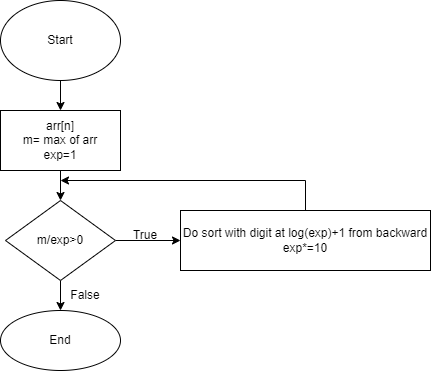
\includegraphics[width=0.5\textwidth]{RadixSort Flowchart}
					\end{figure}
					
				\item \textbf{Description:}
					\begin{enumerate}
					\item Find the largest element in the unsorted input array (Array)
					\item Create a for expression that loops d times, where d = number of digits in the largest element (maxim)
					\item For the first place value, call counting sort, jump place value by 10 to move to the next significant digit
					\item Continue step c for all place values (finish all d passes)
					\end{enumerate}
				
				\item \textbf{Advantage, disadvantage:}
					\begin{table}[H]
						\centering
						\begin{tabular}{|p{8cm}|p{8cm}|}
							\hline
							\textbf{Advantage} & \textbf{Disadvantage} \\
							\hline
							\hline
							As a non-comparison-based sorting algorithm with linear time complexity, radix sort has an advantage over comparative sorting algorithms with O(n logn) as their time complexity.   & For very large numbers or a number system with a wider base, radix sort can perform in linear time; however, the subroutine sort requires larger space for the auxiliary array it uses to sort. This increases the space requirements, making it not ideal for such cases where space is important. (For example, software libraries). \\[12pt]
							Radix sort is also faster when the range of the array elements is relatively narrow, but the count of elements to sort is high. It is also much quicker when the algorithm is being run concurrently on parallel machines. & mplementation of radix sort is different for different data types, and the algorithm depends on digits or letters. Hence, it is less flexible than other sorting algorithms. The implementation has to be re-evaluated and altered based on each data type. \\[12pt]
							Since the radix sort algorithm sorts digit by digit, the number of possible digits is limited to the base of the number system used. This means that it can sort multi-digit numbers (like 15 digit numbers) without increasing the range of digits over which the sorting must be done. The range remains 0 to 9 for numbers in the decimal number system, regardless of number size. This is an advantage since an increased range of digits to sort might decrease the algorithm’s efficiency. & In reality, it doesn't perform well because of the hidden large constant factor involved. For example, when the count of digits is very high, and the number of inputs in the array is very small. And it also takes more space. \\
							\hline
						\end{tabular}
					\end{table}
				\item \textbf{Application:}	
					\begin{itemize}
						\item Radix sort can be applied to data that can be sorted lexicographically, such as words and integers. It is also used for stably sorting strings. 
						\item It is a good option when the algorithm runs on parallel machines, making the sorting faster. To use parallelization, we divide the input into several buckets, enabling us to sort the buckets in parallel, as they are independent of each other. 
						\item It is used for constructing a suffix array. (An array that contains all the possible suffixes of a string in sorted order is called a suffix array).
					\end{itemize}
			\end{enumerate}
			
		\rule{15cm}{0.1cm}
		\subsection{Flash Sort}
		\rule{15cm}{0.1cm}
			\begin{enumerate}[label=\textbf{\arabic*})]
				\item \textbf{Main idea:}
				
					Flash Sort assigns each of the n input elements to one of m buckets, efficiently rearranges the input to place the buckets in the correct order, then sorts each bucket.
				\\[12pt]
				\item \textbf{Complexity Analysis of Flash Sort}
				\begin{itemize}
				\item Flash Sort is a distribution sorting algorithm showing linear computational complexity O(n) for uniformly distributed data sets and relatively little additional memory requirement
                \item Flash Sort is not an in-place algorithm as it has to have a list of buckets. It’s also not stable
                \item As with all bucket sorts, performance depends critically on the balance of the buckets. In the ideal case of a balanced data set, each bucket will be approximately the same size. If the number m of buckets is linear in the input size n, each bucket has a constant size, so sorting a single bucket with an O($n^2$) algorithm like insertion sort has complexity O(1). The running time of the final insertion sorts is therefore O(n)
                \item In the worst-case scenarios where almost all the elements are in a few buckets, the complexity of the algorithm is limited by the performance of the final bucket-sorting method, so degrades to O($n^2$)
                \item If stability is required, it is possible to use a second array so elements can be classified sequentially. However, in this case, the algorithm will require O(n) additional memory
                \end{itemize}
				\item \textbf{Flowchart:}
					\begin{figure}[H]
						\centering 
						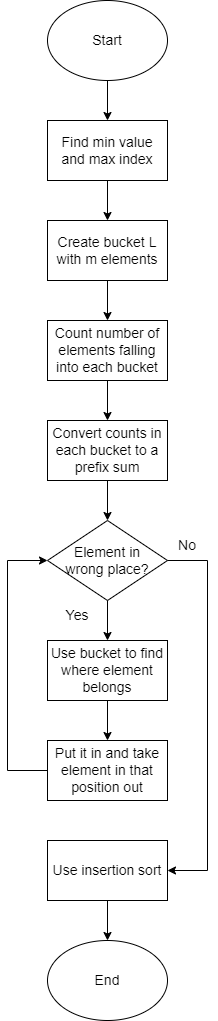
\includegraphics[width=0.2\textwidth]{FlashSortFlowchart}
					\end{figure}
					
				\item \textbf{Description:}
					\begin{itemize}
						\item Step 1: Using a first pass over the input or a priori knowledge, find the minimum and maximum sort keys
                        \item Step 2: Linearly divide the range [amin, amax] into m buckets.
                        \item Step 3: Make one pass over the input, counting the number of elements ai which fall into each bucket
                        \item Step 4: Convert the counts of elements in each bucket to a prefix sum
                        \item Step 5: Rearrange the input to all elements of each bucket
                        \item Step 6: Sort each bucket using insertion sort

					\end{itemize}
				
				\item \textbf{Advantage, disadvantage:}
					\begin{table}[H]
						\centering
						\begin{tabular}{|p{8cm}|p{8cm}|}
							\hline
							\textbf{Advantage} & \textbf{Disadvantage} \\
							\hline
							\hline
							Time complexity of Flash Sort is O(n)  & It’s hard to implement \\[12pt]
							 & It is not stable\\
							\hline
						\end{tabular}
					\end{table}
				\item \textbf{Application:}	
					Flash Sort can be used to sort data, especially the big data size
			\end{enumerate}
	
	\pagebreak
	\flushleft{\section{Experimental results and comments}}
		\subsection{Runtime and Comparisons using in each algorithm presented in table form}
		\begin{table}[H]
		\centering
		\scalebox{0.9}{
		\begin{tabular}{|c|c|c|c|c|c|c|c|c|c|c|c|c|}
		 \hline
		 \multicolumn{ 7}{|c|}{Data Order: Randomized} \\
		 \hline
		 Data Size & \multicolumn{2}{|c|}{10000} & \multicolumn{2}{|c|}{30000} & \multicolumn{2}{|c|}{50000} \\
		 \hline
		 Resulting Statics & Running Time & Comparison & Running Time & Comparison & Running Time & Comparison\\
		 \hline
         Selection Sort & 46.974 & 100009999 & 468.809 & 900029999 & 1296.95 & 2500049999\\ 
         \hline
         Insertion Sort & 31.277 & 50354329 & 312.508 & 450345747 & 860.058 & 1243990628\\
         \hline
         Bubble Sort & 125.078 & 99999837 & 1642.11 & 899917872 & 4787.19 & 2500062365\\ 
         \hline
         Shaker Sort & 125.072 & 75891900 & 1310.84 & 676108631 & 3667.34 & 1871745775\\ 
         \hline
         Shell Sort & 0 & 646268 & 16.05 & 2271877 & 0 & 4551665\\ 
         \hline
         Heap Sort & 0 & 637530 & 15.621 & 2150696 & 0 & 3772710\\ 
         \hline
         Merge Sort & 0 & 583792 & 15.632 & 1937472 & 15.625 & 3383111\\ 
         \hline
         Quick Sort & 0 & 314274 & 15.636 & 1064713 & 0 & 1850433\\ 
         \hline
         Counting Sort & 0 & 90000 & 0 & 270000 & 0 & 415538\\
         \hline
         Radix Sort & 0 & 140056 & 0 & 510070 & 0 & 850070\\
         \hline
		 Flash Sort 	& 0 & 98031 & 0 & 297490 & 0 & 471003\\
		 \hline
		\end{tabular}}
		\caption{Sorting algorithms performance on random data with different range}
		\end{table}
		
		\begin{table}[H]
		\centering
		\scalebox{0.9}{
		\begin{tabular}{|c|c|c|c|c|c|c|c|c|c|c|c|c|}
		 \hline
		 \multicolumn{7}{|c|}{Data Order: Randomized} \\
		 \hline
		 Data Size & \multicolumn{2}{|c|}{100000} & \multicolumn{2}{|c|}{300000} & \multicolumn{2}{|c|}{500000} \\
		 \hline
		 Resulting Statics & Running Time & Comparison & Running Time & Comparison & Running Time & Comparison\\
		 \hline
         Selection Sort  & 5225.03 & 10000099999 & 46814.8 & 90000299999 & 135818 & 250000499999\\ 
         \hline
         Insertion Sort  & 3469.14 & 4982058211 & 31208.9 & 45080012911 & 90324.4 & 125061404569\\ 
         \hline
         Bubble Sort  & 19947.8 & 10000004637 & 186809 & 90000119752 & 544084 & 250000243101\\
         \hline
         Shaker Sort  & 14911.6 & 7473128176 & 135329 & 67642274375 & 393814 & 187618943356\\
         \hline
         Shell Sort  & 15.626 & 9885033 & 62.503 & 34344952 & 109.375 & 66339250\\
         \hline
         Heap Sort  & 15.625 & 8044440 & 62.509 & 26487266 & 125.002 & 45968441\\
         \hline
         Merge Sort  & 31.255 & 7165784 & 78.134 & 23381100 & 120.296 &  40382232\\ 
         \hline
         Quick Sort  & 15.62 & 4123053 & 31.263 & 14600603 & 46.866 & 28417375\\  \hline
         Counting Sort  & 0 & 765538 & 0 & 2165538 & 0 & 3565538\\ 
         \hline
         Radix Sort  & 0 & 1700070 & 15.626 & 5100070 & 15.625 & 8500070\\
         \hline
		 Flash Sort 	& 0 & 893717 & 15.622 & 2747260 & 15.639 & 4731984\\
		 \hline
		\end{tabular}}
		\caption{Sorting algorithms performance on random data with different range}
		\end{table}
		\sectionline
		\begin{table}[H]
		\centering
		\scalebox{0.9}{
		\begin{tabular}{|c|c|c|c|c|c|c|c|c|c|c|c|c|}
		 \hline
		 \multicolumn{ 7}{|c|}{Data Order: Nearly Sorted} \\
		 \hline
		 Data Size & \multicolumn{2}{|c|}{10000} & \multicolumn{2}{|c|}{30000} & \multicolumn{2}{|c|}{50000} \\
		 \hline
		 Resulting Statics & Running Time & Comparison & Running Time & Comparison & Running Time & Comparison\\
		 \hline
         Selection Sort     & 46.951 & 100009999 & 469.473 & 900029999 & 1297.17 & 2500049999\\
         \hline
         Insertion Sort     & 0 & 224046 & 0 & 498842 & 0 & 627518\\
         \hline
         Bubble Sort    & 62.952 & 99799101 & 478.284 & 813532797 & 1094.74 & 1932183440\\
         \hline
         Shaker Sort    & 0 & 299775 & 16.3 & 779831 & 0 & 1499775\\
         \hline
         Shell Sort     & 0 & 418765 & 15.648 & 1320351 & 0 & 2267924\\
         \hline
         Heap Sort      & 0 & 670033 & 15.713 & 2236560 & 0 & 3925314\\
         \hline
         Merge Sort     & 0 & 510502 & 15.626 & 1672259 & 0 & 2806372\\
         \hline
         Quick Sort     & 0 & 5656580 & 15.644 & 24423526 & 31.305 & 88573692\\
         \hline
         Counting Sort  & 0 & 90002 & 0 & 270002 & 0 & 450002\\
         \hline
         Radix Sort     & 0 & 140056 & 0 & 510070 & 0 & 850070\\
         \hline
		 Flash Sort     & 0 & 127958 & 0 & 383964 & 0 & 639962\\
		 \hline
		\end{tabular}}
		\caption{Sorting algorithms performance on nearly sorted data with different range}
		\end{table}
		
		\begin{table}[H]
		\centering
		\scalebox{0.9}{
		\begin{tabular}{|c|c|c|c|c|c|c|c|c|c|c|c|c|}
		 \hline
		 \multicolumn{7}{|c|}{Data Order: Nearly Sorted} \\
		 \hline
		 Data Size & \multicolumn{2}{|c|}{100000} & \multicolumn{2}{|c|}{300000} & \multicolumn{2}{|c|}{500000} \\
		 \hline
		 Resulting Statics & Running Time & Comparison & Running Time & Comparison & Running Time & Comparison\\
		 \hline
         Selection Sort & 5220.22 & 10000099999 & 46746.2 & 90000299999 & 139860 & 250000499999\\ 
         \hline
         Insertion Sort & 0 & 702066 & 0 & 1261482 & 0 & 1838462\\ 
         \hline
         Bubble Sort    & 2242.15 & 3876198465 & 8523.45 & 14930079901 & 10225.2 & 17941060925\\ 
         \hline
         Shaker Sort    & 0 & 2599831 & 0 & 6599879 & 0 & 12999831\\ 
         \hline
         Shell Sort     & 0 & 4659576 & 0 & 15432842 & 15.622 & 25633364\\ 
         \hline
         Heap Sort      & 15.626 & 8365092 & 46.875 & 27413125 & 78.12 & 47404894\\
         \hline
         Merge Sort     & 15.614 & 5854169 & 62.488 & 18747127 & 78.118 & 32106757\\
         \hline
         Quick Sort     & 15.631 & 44582320 & 31.321 & 59386189 & 31.247 & 49849213\\
         \hline
         Counting Sort  & 0 & 900002 & 0 & 2700002 & 0 & 4500002\\ 
         \hline
         Radix Sort     & 0 & 1700070 & 15.635 & 6000084 & 15.9 & 10000084\\
         \hline
		 Flash Sort 	& 0 & 1279964 & 15.631 & 3839962 & 0 & 6399958\\
		 \hline
		\end{tabular}}
		\caption{Sorting algorithms performance on nearly sorted data with different range}
		\end{table}
		\sectionline
		\begin{table}[H]
		\centering
		\scalebox{0.9}{
		\begin{tabular}{|c|c|c|c|c|c|c|c|c|c|c|c|c|}
		 \hline
		 \multicolumn{ 7}{|c|}{Data Order: Sorted} \\
		 \hline
		 Data Size & \multicolumn{2}{|c|}{10000} & \multicolumn{2}{|c|}{30000} & \multicolumn{2}{|c|}{50000} \\
		 \hline
		 Resulting Statics & Running Time & Comparison & Running Time & Comparison & Running Time & Comparison\\
		 \hline
		 Selection Sort & 46.943 & 100009999 & 468.82 & 900029999 & 1298.98 & 2500049999\\
		 \hline
		 Insertion Sort & 0 & 29998 & 0 & 89998 & 0 & 149998\\
		 \hline
		 Bubble Sort 	& 0 & 20001 & 0 & 60001 & 0 & 100001\\
		 \hline
		 Shaker Sort 	& 0 & 19999 & 0 & 59999 & 0 & 99999\\
		 \hline
		 Shell Sort		& 0 & 360042 & 0 & 1170050 & 0 & 2100049\\
		 \hline
		 Heap Sort		& 0 & 670329 & 0 & 2236648 & 3.09 & 3925351\\
		 \hline
		 Merge Sort		& 0 & 475242 & 0 & 1559914 & 0 & 2722826\\
		 \hline
		 Quick Sort		& 0 & 262210 & 0 & 864713 & 0 & 1579403\\
		 \hline
		 Counting Sort 	& 0 & 90002 & 0 & 270002 & 0 & 450002\\
		 \hline
		 Radix Sort 	& 0 & 140056 & 0 & 510070 & 0 & 850070\\
		 \hline
		 Flash Sort 	& 0 & 127992 & 0 & 383992 & 0 & 639992\\
		 \hline
		\end{tabular}}
		\caption{Sorting algorithms performance on sorted data with different range}
		\end{table}
		
		\begin{table}[H]
		\centering
		\scalebox{0.9}{
		\begin{tabular}{|c|c|c|c|c|c|c|c|c|c|c|c|c|}
		 \hline
		 \multicolumn{7}{|c|}{Data Order: Sorted} \\
		 \hline
		 Data Size & \multicolumn{2}{|c|}{100000} & \multicolumn{2}{|c|}{300000} & \multicolumn{2}{|c|}{500000} \\
		 \hline
		 Resulting Statics & Running Time & Comparison & Running Time & Comparison & Running Time & Comparison\\
		 \hline
		 Selection Sort & 5203.17 & 10000099999 & 46669.3 & 90000299999 & 129599 & 250000499999\\
		 \hline
		 Insertion Sort & 0 & 299998 & 0 & 899998 & 0 & 1499998\\
		 \hline
		 Bubble Sort 	& 0 & 200001 & 0 & 600001 & 0 & 1000001\\
		 \hline
		 Shaker Sort 	& 0 & 199999 & 0 & 599999 & 0 & 999999\\
		 \hline
		 Shell Sort		& 0 & 4500051 & 3.91 & 15300061 & 21.92 & 25500058\\
		 \hline
		 Heap Sort		& 15.63 & 8365080 & 46.81 & 27413230 & 93.69 & 47404886\\
		 \hline
		 Merge Sort		& 15.678 & 5745658 & 46.805 & 18645946 & 78.186 & 32017850\\
		 \hline
		 Quick Sort		& 0 & 3358781 & 15.62 & 10709676 & 18.76 & 18335041\\
		 \hline
		 Counting Sort 	& 0 & 900002 & 0 & 2700002 & 0 & 4500002\\
		 \hline
		 Radix Sort 	& 0 & 1700070 & 15.62 & 6000084 & 21.88 & 10000084\\
		 \hline
		 Flash Sort 	& 0 & 1279992 & 0 & 3839992 & 8.456 & 6399992\\
		 \hline
		\end{tabular}}
		\caption{Sorting algorithms performance on sorted data with different range}
		\end{table}
		\sectionline
		\begin{table}[H]
		\centering
		\scalebox{0.9}{
		\begin{tabular}{|c|c|c|c|c|c|c|c|c|c|c|c|c|}
		 \hline
		 \multicolumn{ 7}{|c|}{Data Order: Reversed Sorted} \\
		 \hline
		 Data Size & \multicolumn{2}{|c|}{10000} & \multicolumn{2}{|c|}{30000} & \multicolumn{2}{|c|}{50000} \\
		 \hline
		 Resulting Statics & Running Time & Comparison & Running Time & Comparison & Running Time & Comparison\\
		 \hline
		 Selection Sort & 46.886 & 100009999 & 484.461 & 900029999 & 1375.08 & 2500049999\\
		 \hline
		 Insertion Sort & 62.498 & 100009999 & 609.424 & 900029999 & 1751.52 & 2500049999\\
		 \hline
		 Bubble Sort 	& 144.894 & 100019998 & 1359.45 & 900059998 & 3799.63 & 2500099998\\
		 \hline
		 Shaker Sort 	& 156.323 & 100000000 & 1421.97 & 900000000 & 3925.55 & 2500000000\\
		 \hline
		 Shell Sort		& 0 & 475175 & 0 & 1554051 & 15.639 & 2844628\\
		 \hline
		 Heap Sort		& 0 & 606771 & 0 & 2063324 & 0 & 3612724\\
		 \hline
		 Merge Sort		& 0 & 476441 & 0 & 1573465 & 0 & 2733945\\
		 \hline
		 Quick Sort		& 0 & 493462 & 0 & 1716158 & 0 & 3055462\\
		 \hline
		 Counting Sort 	& 0 & 90002 & 0 & 270002 & 0 & 450002\\
		 \hline
		 Radix Sort 	& 0 & 140056 & 0 & 510070 & 0 & 850070\\
		 \hline
		 Flash Sort 	& 0 & 110501 & 0 & 331501 & 0 & 552501\\
		 \hline
			\end{tabular}}
		\caption{Sorting algorithms performance on reversed sorted data with different range}
		\end{table}
		
		\begin{table}[H]
		\centering
		\scalebox{0.9}{
		\begin{tabular}{|c|c|c|c|c|c|c|c|c|c|c|c|c|}
		 \hline
		 \multicolumn{7}{|c|}{Data Order: Reversed Sorted} \\
		 \hline
		 Data Size & \multicolumn{2}{|c|}{100000} & \multicolumn{2}{|c|}{300000} & \multicolumn{2}{|c|}{500000} \\
		 \hline
		 Resulting Statics & Running Time & Comparison & Running Time & Comparison & Running Time & Comparison\\
		 \hline
		 Selection Sort & 5484.36 & 10000099999 & 49425.7 & 90000299999 & 136486 & 250000499999\\
		 \hline
		 Insertion Sort & 6942.66 & 10000099999 & 70367.8 & 90000299999 & 180954 & 250000499999\\
		 \hline
		 Bubble Sort 	& 14946.1 & 10000199998 & 134832 & 90000599998 & 374753 & 250000999998\\
		 \hline
		 Shaker Sort 	& 15611.4 & 10000000000 & 140205 & 90000000000 & 389069 & 250000000000\\
		 \hline
		 Shell Sort		& 15.699 & 6089190 & 15.637 & 20001852 & 15.687 & 33857581\\
		 \hline
		 Heap Sort		& 15.63 & 7718943 & 46.876 & 25569379 & 94.106 & 44483348
\\
		 \hline
		 Merge Sort		& 15.687 & 5767897 & 46.946 & 18708313 & 78.203 & 32336409\\
		 \hline
		 Quick Sort		& 15.64 & 6610278 & 15.626 & 22138566 & 46.877 & 38720326\\
		 \hline
		 Counting Sort 	& 0 & 900002 & 0 & 2700002 & 0 & 4500002\\
		 \hline
		 Radix Sort 	& 0 & 1700070 & 15.689 & 6000084 & 31.247 & 10000084\\
		 \hline
		 Flash Sort 	& 0 & 1105001 & 0 & 3315001 & 15.626 & 5525001\\
		 \hline
		\end{tabular}}
		\caption{Sorting algorithms performance on reversed sorted data with different range}
		\end{table}
	
		%randomize input
		\pgfplotstableread[row sep=\\,col sep=&]{
		Algorithm 		& 10000 & 30000 & 50000 & 100000 & 300000 & 500000\\
		Selection Sort 	& 100009999   & 900029999  & 2500049999 & 10000099999 & 90000299999 & 250000499999\\
		Insertion Sort 	& 50354329  & 450345747  & 1243990628 & 4982058211 & 45080012911 & 125061404569\\
		Bubble Sort 	& 99999837  & 899917872  & 2500062365 & 10000004637 & 90000119752 & 250000243101\\
		Shaker Sort 	& 75891900  & 676108631  & 1871745775 & 7473128176 & 67642274375 & 187618943356\\
		Shell Sort 		& 646268  & 2271877  & 4551665 & 9885033 & 34344952 & 66339250\\
		}\randomizeDataInput
	
		\pgfplotstableread[row sep=\\,col sep=&]{
		Algorithm 		& 10000 & 30000 & 50000 & 100000 & 300000 & 500000\\
		Heap Sort		& 637530 & 2150696 & 3772710 & 8044440 & 26487266 & 45968441\\
		Merge Sort 		& 583792 & 1937472 & 3383111 & 7165784 & 23381100 & 40382232\\
		Quick Sort 		& 314274 & 1064713 & 1850433 & 4123053 & 14600603 & 28417375\\
		Counting Sort 	& 90000 & 270000 & 415538 & 765538 & 2165538 & 3565538\\
		Radix Sort 		& 140056 & 510070 & 850070 & 1700070 & 5100070 & 8500070\\
		Flash Sort 		& 98031 & 297490 & 471003 & 893717 & 2747260 & 4731984\\
		}\randomizeDataInputt
	
		%Nearly Sorted input
		\pgfplotstableread[row sep=\\,col sep=&]{
		Algorithm 		& 10000 & 30000 & 50000 & 100000 & 300000 & 500000\\
		Selection Sort 	& 100009999 & 900029999 & 2500049999 & 10000099999 & 90000299999 & 250000499999\\
		Insertion Sort 	& 224046 & 498842 & 627518 & 702066 & 1261482 & 1838462\\
		Bubble Sort 	& 99799101 & 813532797 & 1932183440 & 3876198465 & 14930079901 & 17941060925\\
		Shaker Sort 	& 299775 & 779831 & 1499775 & 2599831 & 6599879 & 12999831\\
		Shell Sort 		& 418765 & 1320351 & 2267924 & 4659576 & 15432842 & 25633364\\
		}\nearlySortedInput
	
		\pgfplotstableread[row sep=\\,col sep=&]{
			Algorithm 		& 10000 & 30000 & 50000 & 100000 & 300000 & 500000\\
			Heap Sort		& 670033 & 2236560 & 3925314 & 8365092 & 27413125 & 47404894\\
			Merge Sort 		& 510502 & 1672259 & 2806372 & 5854169 & 18747127 & 32106757\\
			Quick Sort 		& 5656580 & 24423526 & 88573692 & 44582320 & 59386189 & 49849213\\
			Counting Sort 	& 90002 & 270002 & 450002 & 900002 & 2700002 & 4500002\\
			Radix Sort 		& 140056 & 510070 & 850070 & 1700070 & 6000084 & 10000084\\
			Flash Sort 		& 127958 & 383964 & 639962 & 1279964 & 3839962 & 6399958\\
		}\nearlySortedInputt
		
		%Sorted input
		\pgfplotstableread[row sep=\\,col sep=&]{
		Algorithm 		& 10000 & 30000 & 50000 & 100000 & 300000 & 500000\\
		Selection Sort 	& 100009999 & 900029999 & 2500049999 & 10000099999 & 90000299999 & 250000499999\\
		Insertion Sort 	& 29998 & 89998 & 149998 & 299998 & 899998 & 1499998\\
		Bubble Sort 	& 20001 & 60001 & 100001 & 200001 & 600001 & 1000001\\
		Shaker Sort 	& 19999 & 59999 & 99999 & 199999 & 599999 & 999999\\
		Shell Sort 		& 360042 & 1170050 & 2100049 & 4500051 & 15300061 & 25500058\\
		}\sortedInput
	
		\pgfplotstableread[row sep=\\,col sep=&]{
			Algorithm 		& 10000 & 30000 & 50000 & 100000 & 300000 & 500000\\
			Heap Sort		& 670329 & 2236648 & 3925351 & 8365080 & 27413230 & 47404886\\
			Merge Sort 		& 475242 & 1559914 & 2722826 & 5745658 & 18645946 & 32017850\\
			Quick Sort 		& 262210 & 864713 & 1579403 & 3358781 & 10709676 & 18335041\\
			Counting Sort 	& 90002 & 270002 & 450002 & 900002 & 2700002 & 4500002\\
			Radix Sort 		& 140056 & 510070 & 850070 & 1700070 & 6000084 & 10000084\\
			Flash Sort 		& 127992 & 383992 & 639992 & 1279992 & 3839992 & 6399992\\
		}\sortedInputt
		
		%Reversed Sorted input
		\pgfplotstableread[row sep=\\,col sep=&]{
		Algorithm 		& 10000 & 30000 & 50000 & 100000 & 300000 & 500000\\
		Selection Sort 	& 100009999 & 900029999 & 2500049999 & 10000099999 & 90000299999 & 250000499999\\
		Insertion Sort 	& 100009999 & 900029999 & 2500049999 & 10000099999 & 90000299999 & 250000499999\\
		Bubble Sort 	& 100019998 & 900059998 & 2500099998 & 10000199998 & 90000599998 & 250000999998\\
		Shaker Sort 	& 100000000 & 900000000 & 2500000000 & 10000000000 & 90000000000 & 250000000000\\
		Shell Sort 		& 475175 & 1554051 & 2844628 & 6089190 & 20001852 & 33857581\\
		}\reversedSortedInput
	
		\pgfplotstableread[row sep=\\,col sep=&]{
			Algorithm 		& 10000 & 30000 & 50000 & 100000 & 300000 & 500000\\
			Heap Sort		& 606771 & 2063324 & 3612724 & 7718943 & 25569379 & 44483348\\
			Merge Sort 		& 476441 & 1573465 & 2733945 & 5767897 & 18708313 & 32336409\\
			Quick Sort 		& 493462 & 1716158 & 3055462 & 6610278 & 22138566 & 38720326\\
			Counting Sort 	& 90002 & 270002 & 450002 & 900002 & 2700002 & 4500002\\
			Radix Sort 		& 140056 & 510070 & 850070 & 1700070 & 6000084 & 10000084\\
			Flash Sort 		& 110501 & 331501 & 552501 & 1105001 & 3315001 & 5525001\\
		}\reversedSortedInputt
		
	\pagebreak
	\subsection{Runtime and comparisons of each sorting algorithm presented in line chart/ bar chart}
	\centering
	\begin{figure}[H]
	\begin{tikzpicture}
		\begin{axis}
			[
				ylabel={Comparisons},
				title = Randomize Input,
				bar width = 0.3cm,
				ybar,
				y label style={at={(-0.05,0.5)}},
				width=15cm,
				height = 10cm,
				symbolic x coords = {Selection Sort, Insertion Sort, Bubble Sort, Shaker Sort, Shell Sort},
				xtick = data,
				tick label style={font=\tiny},
				tick align=outside,
				grid=both,
				scaled y ticks = false,
				y tick label style={/pgf/number format/fixed},
				tick label style={font=\footnotesize},
				legend image code/.code={
					\draw [/tikz/.cd,bar width=3pt,yshift=-0.2em,bar shift=0pt]
					plot coordinates {(0cm,0.8em)};
				},
				%legend style={inner sep=10pt}, %increase padding legend
				legend style={
					/tikz/every odd column/.style={yshift=2pt},
					/tikz/nodes={text width=55pt,text depth=,anchor=base},
				}
			]
			\addplot[fill=Turquoise] table[x=Algorithm,y=10000]{\randomizeDataInput};
			\addplot[fill=Lavender] table[x=Algorithm,y=30000]{\randomizeDataInput};
			\addplot table[x=Algorithm,y=50000]{\randomizeDataInput};
			\addplot[fill=yellow] table[x=Algorithm,y=100000]{\randomizeDataInput};
			\addplot[fill=WildStrawberry] table[x=Algorithm,y=300000]{\randomizeDataInput};
			\addplot[fill=SeaGreen] table[x=Algorithm,y=500000]{\randomizeDataInput};
			
			\legend{Size: $10^4$, Size: 3.$10^4$, Size: 5.$10^4$, Size: $10^5$, Size: 3.$10^5$, Size: 5.$10^5$}
		\end{axis}
	\end{tikzpicture}
	\caption{Sorting algorithm's comparisons statistics on different range of data}
	\end{figure}
	
	\begin{figure}[H]
	\begin{tikzpicture}
		\begin{axis}
			[
				ylabel={Comparisons},
				title = Randomize Input,
				bar width = 0.2cm,
				ybar,
				y label style={at={(-0.05,0.5)}},
				width=15cm,
				height = 10cm,
				symbolic x coords = {Heap Sort, Merge Sort, Quick Sort, Counting Sort, Radix Sort, Flash Sort},
				xtick = data,
				tick label style={font=\tiny},
				tick align=outside,
				grid=both,
				scaled y ticks = false,
				y tick label style={/pgf/number format/fixed},
				tick label style={font=\footnotesize},
				legend image code/.code={
					\draw [/tikz/.cd,bar width=3pt,yshift=-0.2em,bar shift=0pt]
					plot coordinates {(0cm,0.8em)};
				},
				%legend style={inner sep=10pt}, %increase padding legend
				legend style={
					/tikz/every odd column/.style={yshift=2pt},
					/tikz/nodes={text width=55pt,text depth=,anchor=base},
				}
			]
			\addplot[fill=Turquoise] table[x=Algorithm,y=10000]{\randomizeDataInputt};
			\addplot[fill=Lavender] table[x=Algorithm,y=30000]{\randomizeDataInputt};
			\addplot table[x=Algorithm,y=50000]{\randomizeDataInputt};
			\addplot[fill=yellow] table[x=Algorithm,y=100000]{\randomizeDataInputt};
			\addplot[fill=WildStrawberry] table[x=Algorithm,y=300000]{\randomizeDataInputt};
			\addplot[fill=SeaGreen] table[x=Algorithm,y=500000]{\randomizeDataInputt};
			
			\legend{Size: $10^4$, Size: 3.$10^4$, Size: 5.$10^4$, Size: $10^5$, Size: 3.$10^5$, Size: 5.$10^5$}
		\end{axis}
	\end{tikzpicture}
	\caption{Sorting algorithm's comparisons statistics on different range of data}
	\end{figure}
	
	\begin{figure}[H]
	\begin{tikzpicture}
		\begin{axis}
			[
				ylabel={Comparisons},
				title = Nearly Sorted Input,
				bar width = 0.2cm,
				ybar,
				y label style={at={(-0.05,0.5)}},
				width=15cm,
				height = 10cm,
				symbolic x coords = {Selection Sort, Insertion Sort, Bubble Sort, Shaker Sort, Shell Sort},
				xtick = data,
				tick label style={font=\tiny},
				tick align=outside,
				grid=both,
				scaled y ticks = false,
				y tick label style={/pgf/number format/fixed},
				tick label style={font=\footnotesize},
				legend image code/.code={
					\draw [/tikz/.cd,bar width=3pt,yshift=-0.2em,bar shift=0pt]
					plot coordinates {(0cm,0.8em)};
				},
				%legend style={inner sep=10pt}, %increase padding legend
				legend style={
					/tikz/every odd column/.style={yshift=2pt},
					/tikz/nodes={text width=55pt,text depth=,anchor=base},
				}
			]
			\addplot[fill=Turquoise] table[x=Algorithm,y=10000]{\nearlySortedInput};
			\addplot[fill=Lavender] table[x=Algorithm,y=30000]{\nearlySortedInput};
			\addplot table[x=Algorithm,y=50000]{\nearlySortedInput};
			\addplot[fill=yellow] table[x=Algorithm,y=100000]{\nearlySortedInput};
			\addplot[fill=WildStrawberry] table[x=Algorithm,y=300000]{\nearlySortedInput};
			\addplot[fill=SeaGreen] table[x=Algorithm,y=500000]{\nearlySortedInput};
			
			\legend{Size: $10^4$, Size: 3.$10^4$, Size: 5.$10^4$, Size: $10^5$, Size: 3.$10^5$, Size: 5.$10^5$}
		\end{axis}
	\end{tikzpicture}
	\caption{Sorting algorithm's comparisons statistics on different range of data}
	\end{figure}
	
	\begin{figure}[H]
	\begin{tikzpicture}
		\begin{axis}
			[
				ylabel={Comparisons},
				title = Nearly Sorted Input,
				bar width = 0.2cm,
				ybar,
				y label style={at={(-0.05,0.5)}},
				width=15cm,
				height = 10cm,
				symbolic x coords = {Heap Sort, Merge Sort, Quick Sort, Counting Sort, Radix Sort, Flash Sort},
				xtick = data,
				tick label style={font=\tiny},
				tick align=outside,
				grid=both,
				scaled y ticks = false,
				y tick label style={/pgf/number format/fixed},
				tick label style={font=\footnotesize},
				legend image code/.code={
					\draw [/tikz/.cd,bar width=3pt,yshift=-0.2em,bar shift=0pt]
					plot coordinates {(0cm,0.8em)};
				},
				%legend style={inner sep=10pt}, %increase padding legend
				legend style={
					/tikz/every odd column/.style={yshift=2pt},
					/tikz/nodes={text width=55pt,text depth=,anchor=base},
				}
			]
			\addplot[fill=Turquoise] table[x=Algorithm,y=10000]{\nearlySortedInputt};
			\addplot[fill=Lavender] table[x=Algorithm,y=30000]{\nearlySortedInputt};
			\addplot table[x=Algorithm,y=50000]{\nearlySortedInputt};
			\addplot[fill=yellow] table[x=Algorithm,y=100000]{\nearlySortedInputt};
			\addplot[fill=WildStrawberry] table[x=Algorithm,y=300000]{\nearlySortedInputt};
			\addplot[fill=SeaGreen] table[x=Algorithm,y=500000]{\nearlySortedInputt};
			
			\legend{Size: $10^4$, Size: 3.$10^4$, Size: 5.$10^4$, Size: $10^5$, Size: 3.$10^5$, Size: 5.$10^5$}
		\end{axis}
	\end{tikzpicture}
	\caption{Sorting algorithm's comparisons statistics on different range of data}
	\end{figure}
	
	\begin{figure}[H]
	\begin{tikzpicture}
		\begin{axis}
			[
				ylabel={Comparisons},
				title = Sorted Input,
				bar width = 0.2cm,
				ybar,
				y label style={at={(-0.05,0.5)}},
				width=15cm,
				height = 10cm,
				symbolic x coords = {Selection Sort, Insertion Sort, Bubble Sort, Shaker Sort, Shell Sort},
				xtick = data,
				tick label style={font=\tiny},
				tick align=outside,
				grid=both,
				scaled y ticks = false,
				y tick label style={/pgf/number format/fixed},
				tick label style={font=\footnotesize},
				legend image code/.code={
					\draw [/tikz/.cd,bar width=3pt,yshift=-0.2em,bar shift=0pt]
					plot coordinates {(0cm,0.8em)};
				},
				%legend style={inner sep=10pt}, %increase padding legend
				legend style={
					/tikz/every odd column/.style={yshift=2pt},
					/tikz/nodes={text width=55pt,text depth=,anchor=base},
				}
			]
			\addplot[fill=Turquoise] table[x=Algorithm,y=10000]{\sortedInput};
			\addplot[fill=Lavender] table[x=Algorithm,y=30000]{\sortedInput};
			\addplot table[x=Algorithm,y=50000]{\sortedInput};
			\addplot[fill=yellow] table[x=Algorithm,y=100000]{\sortedInput};
			\addplot[fill=WildStrawberry] table[x=Algorithm,y=300000]{\sortedInput};
			\addplot[fill=SeaGreen] table[x=Algorithm,y=500000]{\sortedInput};
			
			\legend{Size: $10^4$, Size: 3.$10^4$, Size: 5.$10^4$, Size: $10^5$, Size: 3.$10^5$, Size: 5.$10^5$}
		\end{axis}
	\end{tikzpicture}
	\caption{Sorting algorithm's comparisons statistics on different range of data}
	\end{figure}
	
	\begin{figure}[H]
	\begin{tikzpicture}
		\begin{axis}
			[
				ylabel={Comparisons},
				title = Sorted Input,
				bar width = 0.2cm,
				ybar,
				y label style={at={(-0.05,0.5)}},
				width=15cm,
				height = 10cm,
				symbolic x coords = {Heap Sort, Merge Sort, Quick Sort, Counting Sort, Radix Sort, Flash Sort},
				xtick = data,
				tick label style={font=\tiny},
				tick align=outside,
				grid=both,
				scaled y ticks = false,
				y tick label style={/pgf/number format/fixed},
				tick label style={font=\footnotesize},
				legend image code/.code={
					\draw [/tikz/.cd,bar width=3pt,yshift=-0.2em,bar shift=0pt]
					plot coordinates {(0cm,0.8em)};
				},
				%legend style={inner sep=10pt}, %increase padding legend
				legend style={
					/tikz/every odd column/.style={yshift=2pt},
					/tikz/nodes={text width=55pt,text depth=,anchor=base},
				}
			]
			\addplot[fill=Turquoise] table[x=Algorithm,y=10000]{\sortedInputt};
			\addplot[fill=Lavender] table[x=Algorithm,y=30000]{\sortedInputt};
			\addplot table[x=Algorithm,y=50000]{\sortedInputt};
			\addplot[fill=yellow] table[x=Algorithm,y=100000]{\sortedInputt};
			\addplot[fill=WildStrawberry] table[x=Algorithm,y=300000]{\sortedInputt};
			\addplot[fill=SeaGreen] table[x=Algorithm,y=500000]{\sortedInputt};
			
			\legend{Size: $10^4$, Size: 3.$10^4$, Size: 5.$10^4$, Size: $10^5$, Size: 3.$10^5$, Size: 5.$10^5$}
		\end{axis}
	\end{tikzpicture}
	\caption{Sorting algorithm's comparisons statistics on different range of data}
	\end{figure}
	
	\begin{figure}[H]
	\begin{tikzpicture}
		\begin{axis}
			[
				ylabel={Comparisons},
				title = Reversed Sorted Input,
				bar width = 0.2cm,
				ybar,
				y label style={at={(-0.05,0.5)}},
				width=15cm,
				height = 10cm,
				symbolic x coords = {Selection Sort, Insertion Sort, Bubble Sort, Shaker Sort, Shell Sort},
				xtick = data,
				tick label style={font=\tiny},
				tick align=outside,
				grid=both,
				scaled y ticks = false,
				y tick label style={/pgf/number format/fixed},
				tick label style={font=\footnotesize},
				legend image code/.code={
					\draw [/tikz/.cd,bar width=3pt,yshift=-0.2em,bar shift=0pt]
					plot coordinates {(0cm,0.8em)};
				},
				%legend style={inner sep=10pt}, %increase padding legend
				legend style={
					/tikz/every odd column/.style={yshift=2pt},
					/tikz/nodes={text width=55pt,text depth=,anchor=base},
				}
			]
			\addplot[fill=Turquoise] table[x=Algorithm,y=10000]{\reversedSortedInput};
			\addplot[fill=Lavender] table[x=Algorithm,y=30000]{\reversedSortedInput};
			\addplot table[x=Algorithm,y=50000]{\reversedSortedInput};
			\addplot[fill=yellow] table[x=Algorithm,y=100000]{\reversedSortedInput};
			\addplot[fill=WildStrawberry] table[x=Algorithm,y=300000]{\reversedSortedInput};
			\addplot[fill=SeaGreen] table[x=Algorithm,y=500000]{\reversedSortedInput};
			
			\legend{Size: $10^4$, Size: 3.$10^4$, Size: 5.$10^4$, Size: $10^5$, Size: 3.$10^5$, Size: 5.$10^5$}
		\end{axis}
	\end{tikzpicture}
	\caption{Sorting algorithm's comparisons statistics on different range of data}
	\end{figure}
	
	\begin{figure}[H]
	\begin{tikzpicture}
		\begin{axis}
			[
				ylabel={Comparisons},
				title = Reversed Sorted Input,
				bar width = 0.2cm,
				ybar,
				y label style={at={(-0.05,0.5)}},
				width=15cm,
				height = 10cm,
				symbolic x coords = {Heap Sort, Merge Sort, Quick Sort, Counting Sort, Radix Sort, Flash Sort},
				xtick = data,
				tick label style={font=\tiny},
				tick align=outside,
				grid=both,
				scaled y ticks = false,
				y tick label style={/pgf/number format/fixed},
				tick label style={font=\footnotesize},
				legend image code/.code={
					\draw [/tikz/.cd,bar width=3pt,yshift=-0.2em,bar shift=0pt]
					plot coordinates {(0cm,0.8em)};
				},
				%legend style={inner sep=10pt}, %increase padding legend
				legend style={
					/tikz/every odd column/.style={yshift=2pt},
					/tikz/nodes={text width=55pt,text depth=,anchor=base},
				}
			]
			\addplot[fill=Turquoise] table[x=Algorithm,y=10000]{\reversedSortedInputt};
			\addplot[fill=Lavender] table[x=Algorithm,y=30000]{\reversedSortedInputt};
			\addplot table[x=Algorithm,y=50000]{\reversedSortedInputt};
			\addplot[fill=yellow] table[x=Algorithm,y=100000]{\reversedSortedInputt};
			\addplot[fill=WildStrawberry] table[x=Algorithm,y=300000]{\reversedSortedInputt};
			\addplot[fill=SeaGreen] table[x=Algorithm,y=500000]{\reversedSortedInputt};
			
			\legend{Size: $10^4$, Size: 3.$10^4$, Size: 5.$10^4$, Size: $10^5$, Size: 3.$10^5$, Size: 5.$10^5$}
		\end{axis}
	\end{tikzpicture}
	\caption{Sorting algorithm's comparisons statistics on different range of data}
	\end{figure}
	
	%randomized data
	\pgfplotstableread[row sep=\\,col sep=&]{
		Range  & Runtime 	\\
		10000  & 46.974		\\
		30000  & 468.809 	\\
		50000  & 1296.95 	\\
		100000 & 5225.03	\\
		300000 & 46814.8	\\
		500000 & 135818 	\\
	}\randSelectionSort
	
	\pgfplotstableread[row sep=\\,col sep=&]{
		Range  & Runtime 	\\
		10000  & 31.277		\\
		30000  & 312.508 	\\
		50000  & 860.058 	\\
		100000 & 3469.14	\\
		300000 & 31208.9	\\
		500000 & 90324.4 	\\
	}\randInsertionSort
	
	\pgfplotstableread[row sep=\\,col sep=&]{
		Range  & Runtime 	\\
		10000  & 125.078	\\
		30000  & 1642.11 	\\
		50000  & 4787.19 	\\
		100000 & 19947.8	\\
		300000 & 186809		\\
		500000 & 544084 	\\
	}\randBubbleSort
	
	\pgfplotstableread[row sep=\\,col sep=&]{
		Range  & Runtime 	\\
		10000  & 125.072	\\
		30000  & 1310.84 	\\
		50000  & 3667.34 	\\
		100000 & 14911.6	\\
		300000 & 135329 	\\
		500000 & 393814 	\\
	}\randShakerSort
	
	\pgfplotstableread[row sep=\\,col sep=&]{
		Range  & Runtime 	\\
		10000  & 0			\\
		30000  & 16.25  	\\
		50000  & 0       	\\
		100000 & 15.626		\\
		300000 & 62.503		\\
		500000 & 109.375 	\\
	}\randShellSort
	
	\pgfplotstableread[row sep=\\,col sep=&]{
		Range  & Runtime 	\\
		10000  & 0			\\
		30000  & 15.621		\\
		50000  & 0  		\\
		100000 & 15.625		\\
		300000 & 62.509		\\
		500000 & 125.002 	\\
	}\randHeapSort
	
	\pgfplotstableread[row sep=\\,col sep=&]{
		Range  & Runtime 	\\
		10000  & 0			\\
		30000  & 15.632    	\\
		50000  & 15.625		\\
		100000 & 31.255		\\
		300000 & 78.134 	\\
		500000 & 120.296 	\\
	}\randMergeSort
	
	\pgfplotstableread[row sep=\\,col sep=&]{
		Range  & Runtime 	\\
		10000  & 0			\\
		30000  & 15.636 	\\
		50000  & 0			\\
		100000 & 15.62		\\
		300000 & 31.263		\\
		500000 & 46.866		\\
	}\randQuickSort
	
	\pgfplotstableread[row sep=\\,col sep=&]{
		Range  & Runtime 	\\
		10000  & 0			\\
		30000  & 0 			\\
		50000  & 0			\\
		100000 & 0			\\
		300000 & 0			\\
		500000 & 0   		\\
	}\randCountingSort
	
	\pgfplotstableread[row sep=\\,col sep=&]{
		Range  & Runtime 	\\
		10000  & 0			\\
		30000  & 0 			\\
		50000  & 0			\\
		100000 & 0			\\
		300000 & 15.626		\\
		500000 & 15.625		\\
	}\randRadixSort
	
	\pgfplotstableread[row sep=\\,col sep=&]{
		Range  & Runtime 	\\
		10000  & 0			\\
		30000  & 0 			\\
		50000  & 0			\\
		100000 & 0			\\
		300000 & 15.622		\\
		500000 & 15.639 	\\
	}\randFlashSort
	
	%Nearly Sorted data
	\pgfplotstableread[row sep=\\,col sep=&]{
		Range  & Runtime 	\\
		10000  & 46.951		\\
		30000  & 469.473 	\\
		50000  & 1297.17 	\\
		100000 & 5220.22	\\
		300000 & 46746.2	\\
		500000 & 139860 	\\
	}\nsortedSelectionSort
	
	\pgfplotstableread[row sep=\\,col sep=&]{
		Range  & Runtime 	\\
		10000  & 0		    \\
		30000  & 0 	        \\
		50000  & 0 	        \\
		100000 & 0	        \\
		300000 & 0	        \\
		500000 & 0 	        \\
	}\nsortedInsertionSort
	
	\pgfplotstableread[row sep=\\,col sep=&]{
		Range  & Runtime 	\\
		10000  & 62.952		\\
		30000  & 478.284 	\\
		50000  & 1094.74 	\\
		100000 & 2242.15	\\
		300000 & 8523.45	\\
		500000 & 10225.2 	\\
	}\nsortedBubbleSort
	
	\pgfplotstableread[row sep=\\,col sep=&]{
		Range  & Runtime 	\\
		10000  & 0		    \\
		30000  & 16.3       \\
		50000  & 0 	        \\
		100000 & 0	        \\
		300000 & 0  		\\
		500000 & 0         	\\
	}\nsortedShakerSort
	
	\pgfplotstableread[row sep=\\,col sep=&]{
		Range  & Runtime 	\\
		10000  & 0			\\
		30000  & 15.648		\\
		50000  & 0 		    \\
		100000 & 0		    \\
		300000 & 0  		\\
		500000 & 15.622 	\\
	}\nsortedShellSort
	
	\pgfplotstableread[row sep=\\,col sep=&]{
		Range  & Runtime 	\\
		10000  & 0			\\
		30000  & 15.713		\\
		50000  & 0 		    \\
		100000 & 15.626		\\
		300000 & 46.875		\\
		500000 & 78.12   	\\
	}\nsortedHeapSort
	
	\pgfplotstableread[row sep=\\,col sep=&]{
		Range  & Runtime 	\\
		10000  & 0  		\\
		30000  & 15.626    	\\
		50000  & 0  		\\
		100000 & 15.614 	\\
		300000 & 62.488 	\\
		500000 & 78.118 	\\
	}\nsortedMergeSort
	
	\pgfplotstableread[row sep=\\,col sep=&]{
		Range  & Runtime 	\\
		10000  & 0			\\
		30000  & 15.644		\\
		50000  & 31.305		\\
		100000 & 15.631		\\
		300000 & 31.321		\\
		500000 & 31.247 	\\
	}\nsortedQuickSort
	
	\pgfplotstableread[row sep=\\,col sep=&]{
		Range  & Runtime 	\\
		10000  & 0			\\
		30000  & 0 			\\
		50000  & 0			\\
		100000 & 0			\\
		300000 & 0			\\
		500000 & 0       	\\
	}\nsortedCountingSort
	
	\pgfplotstableread[row sep=\\,col sep=&]{
		Range  & Runtime 	\\
		10000  & 0			\\
		30000  & 0 			\\
		50000  & 0			\\
		100000 & 0			\\
		300000 & 15.635		\\
		500000 & 15.9    	\\
	}\nsortedRadixSort
	
	\pgfplotstableread[row sep=\\,col sep=&]{
		Range  & Runtime 	\\
		10000  & 0			\\
		30000  & 0 			\\
		50000  & 0			\\
		100000 & 0			\\
		300000 & 15.631		\\
		500000 & 0 	        \\
	}\nsortedFlashSort
	
	%Sorted data
	\pgfplotstableread[row sep=\\,col sep=&]{
		Range  & Runtime 	\\
		10000  & 46.943 	\\
		30000  & 468.82 	\\
		50000  & 1298.98 	\\
		100000 & 5203.17	\\
		300000 & 46669.3	\\
		500000 & 129599 	\\
	}\sortedSelectionSort
	
	\pgfplotstableread[row sep=\\,col sep=&]{
		Range  & Runtime 	\\
		10000  & 0  		\\
		30000  & 0       	\\
		50000  & 0       	\\
		100000 & 0      	\\
		300000 & 0      	\\
		500000 & 0       	\\
	}\sortedInsertionSort
	
	\pgfplotstableread[row sep=\\,col sep=&]{
		Range  & Runtime 	\\
		10000  & 0  		\\
		30000  & 0       	\\
		50000  & 0       	\\
		100000 & 0      	\\
		300000 & 0  		\\
		500000 & 0       	\\
	}\sortedBubbleSort
	
	\pgfplotstableread[row sep=\\,col sep=&]{
		Range  & Runtime 	\\
		10000  & 0     		\\
		30000  & 0       	\\
		50000  & 0       	\\
		100000 & 0      	\\
		300000 & 0      	\\
		500000 & 0      	\\
	}\sortedShakerSort
	
	\pgfplotstableread[row sep=\\,col sep=&]{
		Range  & Runtime 	\\
		10000  & 0			\\
		30000  & 0   		\\
		50000  & 0   		\\
		100000 & 0  		\\
		300000 & 3.91		\\
		500000 & 21.92   	\\
	}\sortedShellSort
	
	\pgfplotstableread[row sep=\\,col sep=&]{
		Range  & Runtime 	\\
		10000  & 0			\\
		30000  & 0   		\\
		50000  & 3.09 		\\
		100000 & 15.63		\\
		300000 & 46.81		\\
		500000 & 93.69   	\\
	}\sortedHeapSort
	
	\pgfplotstableread[row sep=\\,col sep=&]{
		Range  & Runtime 	\\
		10000  & 0			\\
		30000  & 0      	\\
		50000  & 0   		\\
		100000 & 15.678		\\
		300000 & 46.805 	\\
		500000 & 78.186 	\\
	}\sortedMergeSort
	
	\pgfplotstableread[row sep=\\,col sep=&]{
		Range  & Runtime 	\\
		10000  & 0			\\
		30000  & 0 			\\
		50000  & 0			\\
		100000 & 0  		\\
		300000 & 15.62		\\
		500000 & 18.76 		\\
	}\sortedQuickSort
	
	\pgfplotstableread[row sep=\\,col sep=&]{
		Range  & Runtime 	\\
		10000  & 0			\\
		30000  & 0 			\\
		50000  & 0			\\
		100000 & 0			\\
		300000 & 0			\\
		500000 & 0   		\\
	}\sortedCountingSort
	
	\pgfplotstableread[row sep=\\,col sep=&]{
		Range  & Runtime 	\\
		10000  & 0			\\
		30000  & 0 			\\
		50000  & 0			\\
		100000 & 0			\\
		300000 & 15.62		\\
		500000 & 21.88 		\\
	}\sortedRadixSort
	
	\pgfplotstableread[row sep=\\,col sep=&]{
		Range  & Runtime 	\\
		10000  & 0			\\
		30000  & 0 			\\
		50000  & 0			\\
		100000 & 0			\\
		300000 & 0  		\\
		500000 & 8.456		\\
	}\sortedFlashSort
	
	
	%Reverse Sorted data
	\pgfplotstableread[row sep=\\,col sep=&]{
		Range  & Runtime 	\\
		10000  & 46.886		\\
		30000  & 484.461 	\\
		50000  & 1375.08 	\\
		100000 & 5484.36	\\
		300000 & 49425.7	\\
		500000 & 136486 	\\
	}\revSelectionSort
	
	\pgfplotstableread[row sep=\\,col sep=&]{
		Range  & Runtime 	\\
		10000  & 62.498		\\
		30000  & 609.424 	\\
		50000  & 1751.52 	\\
		100000 & 6942.66	\\
		300000 & 70367.8	\\
		500000 & 180954 	\\
	}\revInsertionSort
	
	\pgfplotstableread[row sep=\\,col sep=&]{
		Range  & Runtime 	\\
		10000  & 144.894	\\
		30000  & 1359.45 	\\
		50000  & 3799.63 	\\
		100000 & 14946.1	\\
		300000 & 134832		\\
		500000 & 374753 	\\
	}\revBubbleSort
	
	\pgfplotstableread[row sep=\\,col sep=&]{
		Range  & Runtime 	\\
		10000  & 156.323	\\
		30000  & 1421.97 	\\
		50000  & 3925.55 	\\
		100000 & 15611.4	\\
		300000 & 140205		\\
		500000 & 389069 	\\
	}\revShakerSort
	
	\pgfplotstableread[row sep=\\,col sep=&]{
		Range  & Runtime 	\\
		10000  & 0			\\
		30000  & 0   		\\
		50000  & 15.639 	\\
		100000 & 15.699		\\
		300000 & 15.637		\\
		500000 & 15.687 	\\
	}\revShellSort
	
	\pgfplotstableread[row sep=\\,col sep=&]{
		Range  & Runtime 	\\
		10000  & 0			\\
		30000  & 0   		\\
		50000  & 0   		\\
		100000 & 15.63		\\
		300000 & 46.876		\\
		500000 & 94.106 	\\
	}\revHeapSort
	
	\pgfplotstableread[row sep=\\,col sep=&]{
		Range  & Runtime 	\\
		10000  & 0			\\
		30000  & 0      	\\
		50000  & 0   		\\
		100000 & 15.687	    \\
		300000 & 46.946  	\\
		500000 & 78.203  	\\
	}\revMergeSort
	
	\pgfplotstableread[row sep=\\,col sep=&]{
		Range  & Runtime 	\\
		10000  & 0			\\
		30000  & 0 			\\
		50000  & 0			\\
		100000 & 15.64		\\
		300000 & 15.626		\\
		500000 & 46.877		\\
	}\revQuickSort
	
	\pgfplotstableread[row sep=\\,col sep=&]{
		Range  & Runtime 	\\
		10000  & 0			\\
		30000  & 0 			\\
		50000  & 0			\\
		100000 & 0			\\
		300000 & 0			\\
		500000 & 0   		\\
	}\revCountingSort
	
	\pgfplotstableread[row sep=\\,col sep=&]{
		Range  & Runtime 	\\
		10000  & 0			\\
		30000  & 0 			\\
		50000  & 0			\\
		100000 & 0			\\
		300000 & 15.689		\\
		500000 & 31.247		\\
	}\revRadixSort
	
	\pgfplotstableread[row sep=\\,col sep=&]{
		Range  & Runtime 	\\
		10000  & 0			\\
		30000  & 0 			\\
		50000  & 0			\\
		100000 & 0			\\
		300000 & 0  		\\
		500000 & 15.626		\\
	}\revFlashSort
	
	\begin{figure}[H]
	\begin{tikzpicture}
		\begin{axis}
			[
				ylabel={Runtime},
				xlabel={Data Range},
				title = Randomize Input,
				y label style={at={(-0.05,0.5)}},
				width=15cm,
				height = 10cm,
				symbolic x coords = {10000, 30000, 50000, 100000, 300000, 500000},
				xtick = data,
				tick label style={font=\tiny},
				tick align=outside,
				grid=both,
				scaled y ticks = false,
				y tick label style={/pgf/number format/fixed},
				tick label style={font=\footnotesize},
				legend cell align={left},
				%legend style={inner sep=10pt}, %increase padding legend
				legend pos=north west,
				line width=0.65pt,
			]
			\addplot[Blue,mark=square*] table[x=Range,y=Runtime]{\randSelectionSort};
			\addplot[Brown,mark=square*] table[x=Range,y=Runtime]{\randInsertionSort};
			\addplot[Cerulean,mark=square*] table[x=Range,y=Runtime]{\randBubbleSort};
			\addplot[Mulberry,mark=square*] table[x=Range,y=Runtime]{\randShakerSort};
			\addplot[Red,mark=square*] table[x=Range,y=Runtime]{\randShellSort};
			\addplot[YellowOrange,mark=square*] table[x=Range,y=Runtime]{\randHeapSort};
			\addplot[Green,mark=square*] table[x=Range,y=Runtime]{\randMergeSort};
			\addplot[Violet,mark=square*] table[x=Range,y=Runtime]{\randQuickSort};
			\addplot[BrickRed,mark=square*] table[x=Range,y=Runtime]{\randCountingSort};
			\addplot[RoyalPurple,mark=square*] table[x=Range,y=Runtime]{\randRadixSort};
			\addplot[Peach,mark=square*] table[x=Range,y=Runtime]{\randFlashSort};
			\legend{SelectionSort, Insertion Sort, Bubble Sort, Shaker Sort, Shell Sort, Heap Sort, Merge Sort, Quick Sort, Counting Sort, Radix Sort, Flash Sort}
		\end{axis}
	\end{tikzpicture}
	\caption{Sorting algorithm's runtime statistics on different range of data}
	\end{figure}
	
	\begin{figure}[H]
	\begin{tikzpicture}
		\begin{axis}
			[
				ylabel={Runtime},
				xlabel={Data Range},
				title = Nearly Sorted Input,
				y label style={at={(-0.05,0.5)}},
				width=15cm,
				height = 10cm,
				symbolic x coords = {10000, 30000, 50000, 100000, 300000, 500000},
				xtick = data,
				tick label style={font=\tiny},
				tick align=outside,
				grid=both,
				scaled y ticks = false,
				y tick label style={/pgf/number format/fixed},
				tick label style={font=\footnotesize},
				legend cell align={left},
				%legend style={inner sep=10pt}, %increase padding legend
				legend pos=north west,
				line width=0.65pt,
			]
			\addplot[Blue,mark=square*] table[x=Range,y=Runtime]{\nsortedSelectionSort};
			\addplot[Brown,mark=square*] table[x=Range,y=Runtime]{\nsortedInsertionSort};
			\addplot[Cerulean,mark=square*] table[x=Range,y=Runtime]{\nsortedBubbleSort};
			\addplot[Mulberry,mark=square*] table[x=Range,y=Runtime]{\nsortedShakerSort};
			\addplot[Red,mark=square*] table[x=Range,y=Runtime]{\nsortedShellSort};
			\addplot[YellowOrange,mark=square*] table[x=Range,y=Runtime]{\nsortedHeapSort};
			\addplot[Green,mark=square*] table[x=Range,y=Runtime]{\nsortedMergeSort};
			\addplot[Violet,mark=square*] table[x=Range,y=Runtime]{\nsortedQuickSort};
			\addplot[BrickRed,mark=square*] table[x=Range,y=Runtime]{\nsortedCountingSort};
			\addplot[RoyalPurple,mark=square*] table[x=Range,y=Runtime]{\nsortedRadixSort};
			\addplot[Peach,mark=square*] table[x=Range,y=Runtime]{\nsortedFlashSort};
			\legend{SelectionSort, Insertion Sort, Bubble Sort, Shaker Sort, Shell Sort, Heap Sort, Merge Sort, Quick Sort, Counting Sort, Radix Sort, Flash Sort}
		\end{axis}
	\end{tikzpicture}
	\caption{Sorting algorithm's runtime statistics on different range of data}
	\end{figure}
	
	\begin{figure}[H]
	\begin{tikzpicture}
		\begin{axis}
			[
				ylabel={Runtime},
				xlabel={Data Range},
				title = Sorted Input,
				y label style={at={(-0.05,0.5)}},
				width=15cm,
				height = 10cm,
				symbolic x coords = {10000, 30000, 50000, 100000, 300000, 500000},
				xtick = data,
				tick label style={font=\tiny},
				tick align=outside,
				grid=both,
				scaled y ticks = false,
				y tick label style={/pgf/number format/fixed},
				tick label style={font=\footnotesize},
				legend cell align={left},
				%legend style={inner sep=10pt}, %increase padding legend
				legend pos=north west,
				line width=0.65pt,
			]
			\addplot[Blue,mark=square*] table[x=Range,y=Runtime]{\sortedSelectionSort};
			\addplot[Brown,mark=square*] table[x=Range,y=Runtime]{\sortedInsertionSort};
			\addplot[Cerulean,mark=square*] table[x=Range,y=Runtime]{\sortedBubbleSort};
			\addplot[Mulberry,mark=square*] table[x=Range,y=Runtime]{\sortedShakerSort};
			\addplot[Red,mark=square*] table[x=Range,y=Runtime]{\sortedShellSort};
			\addplot[YellowOrange,mark=square*] table[x=Range,y=Runtime]{\sortedHeapSort};
			\addplot[Green,mark=square*] table[x=Range,y=Runtime]{\sortedMergeSort};
			\addplot[Violet,mark=square*] table[x=Range,y=Runtime]{\sortedQuickSort};
			\addplot[BrickRed,mark=square*] table[x=Range,y=Runtime]{\sortedCountingSort};
			\addplot[RoyalPurple,mark=square*] table[x=Range,y=Runtime]{\sortedRadixSort};
			\addplot[Peach,mark=square*] table[x=Range,y=Runtime]{\sortedFlashSort};
			\legend{SelectionSort, Insertion Sort, Bubble Sort, Shaker Sort, Shell Sort, Heap Sort, Merge Sort, Quick Sort, Counting Sort, Radix Sort, Flash Sort}
		\end{axis}
	\end{tikzpicture}
	\caption{Sorting algorithm's runtime statistics on different range of data}
	\end{figure}
	
	\begin{figure}[H]
	\begin{tikzpicture}
		\begin{axis}
			[
				ylabel={Runtime},
				xlabel={Data Range},
				title = Reversed Sorted Input,
				y label style={at={(-0.05,0.5)}},
				width=15cm,
				height = 10cm,
				symbolic x coords = {10000, 30000, 50000, 100000, 300000, 500000},
				xtick = data,
				tick label style={font=\tiny},
				tick align=outside,
				grid=both,
				scaled y ticks = false,
				y tick label style={/pgf/number format/fixed},
				tick label style={font=\footnotesize},
				legend cell align={left},
				%legend style={inner sep=10pt}, %increase padding legend
				legend pos=north west,
				line width=0.65pt,
			]
			\addplot[Blue,mark=square*] table[x=Range,y=Runtime]{\revSelectionSort};
			\addplot[Brown,mark=square*] table[x=Range,y=Runtime]{\revInsertionSort};
			\addplot[Cerulean,mark=square*] table[x=Range,y=Runtime]{\revBubbleSort};
			\addplot[Mulberry,mark=square*] table[x=Range,y=Runtime]{\revShakerSort};
			\addplot[Red,mark=square*] table[x=Range,y=Runtime]{\revShellSort};
			\addplot[YellowOrange,mark=square*] table[x=Range,y=Runtime]{\revHeapSort};
			\addplot[Green,mark=square*] table[x=Range,y=Runtime]{\revMergeSort};
			\addplot[Violet,mark=square*] table[x=Range,y=Runtime]{\revQuickSort};
			\addplot[BrickRed,mark=square*] table[x=Range,y=Runtime]{\revCountingSort};
			\addplot[RoyalPurple,mark=square*] table[x=Range,y=Runtime]{\revRadixSort};
			\addplot[Peach,mark=square*] table[x=Range,y=Runtime]{\revFlashSort};
			\legend{SelectionSort, Insertion Sort, Bubble Sort, Shaker Sort, Shell Sort, Heap Sort, Merge Sort, Quick Sort, Counting Sort, Radix Sort, Flash Sort}
		\end{axis}
	\end{tikzpicture}
	\caption{Sorting algorithm's runtime statistics on different range of data}
	\end{figure}
	\flushleft{
	\subsection{Summary}
	    \begin{enumerate}
	        \item \textbf{Runtime}
	            \begin{itemize}
	                \item Randomized 
	                \begin{itemize}
	                    \item Counting Sort is the best option with big randomized data size, it takes approximately 0 milisecond at size 500,000
	                    \item Bubble Sort is the worst option, it takes up to 544084 ms to sort a randomized array at size 500,000
	                \end{itemize}
	                \item Nearly Sorted
	                \begin{itemize}
	                    \item Insertion Sort, Shaker Sort, Counting Sort, Flash Sort are the best option when the array is nearly sorted, it takes approximately 0 milisecond at size 500,000
	                    \item Selection Sort is the worst option, it takes up to 139860 ms to sort a nearly sorted array at size 500,000
	                \end{itemize}
	                \item Sorted
	                \begin{itemize}
	                    \item Insertion Sort, Bubble Sort, Shaker Sort and Counting Sort are the best option in case that the array is already sorted, they take approximately 0 milisecond at size 500,000
	                    \item Selection Sort is the worst option, it takes up to 129599 ms to run with an array at size 500,000
	                \end{itemize}
	                \item Reversed Sorted
	                \begin{itemize}
	                    \item Counting Sort is the best option with a reversed sorted array, it takes approximately 0 milisecond at size 500,000
	                    \item Bubble Sort and Shaker Sort are the worst option, they take about 380000 ms to sort a reversed sorted array at size 500,000
	                \end{itemize}
	            \end{itemize}
	        \item \textbf{Comparisons}
	            \begin{itemize}
	                \item Randomized 
	                \begin{itemize}
	                    \item Counting Sort is the best option with lowest comparisons, it only compares 3,565,538 times to make a randomized array at size 500,000 sorted
	                    \item Selection Sort and Bubble Sort are the worst option, they have to compare about 250,000,000,000 times to sort a randomized array at size 500,000
	                \end{itemize}
	                \item Nearly Sorted
	                \begin{itemize}
	                    \item Insertion Sort is the best option with lowest comparisons, it only compares 1,838,462 times to sort a nearly sorted array at size 500,000
	                    \item Selection Sort is the worst option, it has to compare 250,000,499,999 times to sort an array which is nearly sorted at size 500,000
	                \end{itemize}
	                \item Sorted
	                \begin{itemize}
	                    \item Bubble Sort and Shaker Sort are the best option with lowest comparisons, it only compares about 1,000,000 times to traverse and know that the array at size 500,000 is already sorted
	                    \item Selection Sort is the worst option, it has to compare about 250,000,499,999 times to make sure that the array at size 500,000 is sorted
	                \end{itemize}
	                \item Reversed Sorted
	                \begin{itemize}
	                    \item Counting Sort is the best option with lowest comparisons, it only compares about 4,500,002 times to make a reversed sorted array at size 500,000 sorted
	                    \item Selection Sort, Insertion Sort, Bubble Sort, Shaker Sort are the worst option, it have to compare about 250,000,000,000 times to sort an array at size 500,000 if it is reversed sorted
	                \end{itemize}
	            \end{itemize}
	    \end{enumerate}
	
	}
	
	\pagebreak
	\flushleft{
	\section{Project organization and Programming notes}
	\begin{enumerate}
	    \item \textbf{File}
	        \begin{itemize}
	            \item \textbf{main.cpp}
	            
	                This file contains all the functions for user to see the runtime and comparisons from a sorting algorithm or user want to compare 2 algorithm simultaneously. When user input command from terminal, this file will call sorting function from Sorting Algorithm.h to sort the input which generated from DataGenerator.h and then print the runtime or comparisons on terminal.
	            \item \textbf{DataGenerator.cpp}
	                
	                This file generates input in specific order(random, nearly sorted, sorted, reversed sorted) with specific range(10000, 30000, 50000, 100000, 300000, 500000).
	            \item \textbf{SortingAlgorithm.h}
	            
	                This file includes all the name of sorting functions(Merge sort, Quick Sort, Heap Sort,...).
	           \item \textbf{Sorting.cpp}
	           
	                Include detail the implementation of each sorting functions
	        \end{itemize}
	    \item \textbf{Function}
	        \begin{itemize}
	            \item \textbf{double time-"Algorithm"(int a[], int n)}: 
	            
	                Ex: double time-bubble-sort: get runtime of bubble sort.
	            \item \textbf{long long comp-"Algorithm"(int a[], int n)}: 
	            
	                Ex: long long comp-bubble-sort: return number of comparisons of Bubble Sort.
	            \item \textbf{void algorithmMode(vector<string> argv)}: go to algorithm mode.
	            \item\textbf{void compareMode(vector<string> argv)}: go to compare mode.
	            \item\textbf{void command1(vector<string> argv)}: Run a sorting algorithm on the given input data
	            \item\textbf{void command2(vector<string> argv)}: Run a sorting algorithm on the data generated automatically with specified
size and order
                \item\textbf{void command3(vector<string> argv)}: Run a sorting algorithm on ALL data arrangements of a specified size.
                \item\textbf{void command4(vector<string> argv)}: Run two sorting algorithms on the given input.
                \item\textbf{void command5(vector<string> argv)}: Run two sorting algorithms on the data generated automatically
	        \end{itemize}
	    \item \textbf{Library}
	    
	        \textbf{std::chrono library}
	        
	            Used for getting the runtime of a sorting function in milisecond.
	            
	\end{enumerate}
	\addcontentsline{toc}{section}{References}
	}
	\begin{thebibliography}{}
		\bibitem{} \href{https://www.codeproject.com/Questions/164306/convert-argv-to-something-and-back}{Convert argv to something and back}
		\bibitem{} \href{https://www.tutorialspoint.com/data_structures_algorithms/selection_sort_algorithm.htm}{Selection Sort Pseudocode}
		\bibitem{} \href{https://techvidvan.com/tutorials/selection-sort/}{Steps, Pseudocode of Selection Sort}
		\bibitem{} \href {http://csir.org.gh/images/Doc/Refereed_Journal_Articles/Improved%20Selection%20Sort%20Algorithm.pdf}{Main idea of Selection Sort}
		\bibitem{} \href{https://www.liquisearch.com/selection_sort/variants}{Selection Sort Variants}
		\bibitem{} \href{https://dbmspoly.blogspot.com/p/advantage-disadvantages-of-sort.html}{Selection Sort Advantage/ Disadvantage}
		\bibitem{} \href{https://iq.opengenus.org/selection-sort/}{Application of Selection Sort}
		\bibitem{} \href{https://www.simplilearn.com/tutorials/data-structure-tutorial/selection-sort-algorithm#the_complexity_of_selection_sort_algorithm}{Complexity Analysis of Selection Sort}
		\bibitem{} \href{https://www.mygreatlearning.com/blog/bubble-sort/#sh11}{Bubble Sort Pseudocode}
		\bibitem{} \href{https://en.wikipedia.org/wiki/Bubble_sort}{Bubble Sort Idea}
		\bibitem{} \href{https://www.geeksforgeeks.org/bubble-sort/}{Bubble Sort Source Code}
		\bibitem{} \href{http://dbmspoly.blogspot.com/p/advantage-disadvantages-of-sort.html}{Shaker Sort Advantage Disadvantage}
		\bibitem{} \href{https://www.geeksforgeeks.org/cocktail-sort/}{Cocktail/ Shaker Sort}
		\bibitem{} \href{https://iq.opengenus.org/cocktail-shaker-sort/}{Cocktail/ Shaker Sort Pseudocode}
		\bibitem{} \href{https://en.wikipedia.org/wiki/Cocktail_shaker_sort}{Cocktail/ Shaker Sort}
		\bibitem{} \href{https://www.tutorialspoint.com/data_structures_algorithms/shell_sort_algorithm.htm}{Shell Sort Pseudocode}
		\bibitem{} \href{https://en.wikipedia.org/wiki/Shellsort}{Shell Sort Idea}
		\bibitem{} \href{https://www.geeksforgeeks.org/shellsort/}{Shell Sort Source Code, Idea, Variant}
		\bibitem{} \href{https://www.tutorialspoint.com/Heap-Sort}{Main Idea Heap Sort}
		\bibitem{} \href{https://www.liquisearch.com/heapsort/variations}{Heap Sort Variants}
		\bibitem{} \href{https://www.quora.com/What-are-the-benefits-of-heap-sort-and-its-disadvantages-compared-to-other-sorting-algorithms}{Advantage and Disadvantage of Heap Sort}
		\bibitem{} \href{https://fullyunderstood.com/pseudocodes/heap-sort/}{Heap Sort Pseudocode}
		\bibitem{} \href{https://www.interviewkickstart.com/learn/heap-sort#:~:text=Applications%20of%20Heap%20Sort,-Implementation%20of%20priority&text=Because%20algorithms%20like%20merge%20sort,an%20almost%20sorted%20array%2C%20etc.}{Apllications, Complexity Analysis of Heap Sort}
		\bibitem{} \href{https://www.geeksforgeeks.org/merge-sort/}{Main Idea}
		\bibitem{} \href{https://iq.opengenus.org/insertion-sort/#:~:text=A%20variant%20named%20binary%20merge,on%20a%20linked%20list%20structure}{Variants of Merge Sort}
		\bibitem{} \href{http://dbmspoly.blogspot.com/p/advantage-disadvantages-of-sort.html}{Advantage and Disadvantage of Merge Sort}
		\bibitem{} \href{https://www.tutorialspoint.com/data_structures_algorithms/merge_sort_algorithm.htm}{Advantage and Disadvantage of Merge Sort}
		\bibitem{} \href{https://en.wikipedia.org/wiki/Quicksort}{Quick Sort Main Idea}
		\bibitem{} \href{https://www.geeksforgeeks.org/quick-sort/}{Quick Sort Source Code}
		\bibitem{} \href{https://www.mygreatlearning.com/blog/quick-sort-algorithm/}{Quick Sort Pseudocode}
		\bibitem{} \href{https://www.geeksforgeeks.org/counting-sort/}{Counting Sort Idea}
		\bibitem{} \href{https://www.simplilearn.com/tutorials/data-structure-tutorial/counting-sort-algori	thm#:~:text=Applications%20of%20Counting%20Sort%20Algorithm&text=It%20has%20an%20O(n,using%20partial%20hashing%20(1).}{Applications, Complexity Analysis of Counting Sort}
		\bibitem{} \href{https://www.interviewkickstart.com/learn/counting-sort}{Advantage/ Disadvantage of Counting Sort}
		\bibitem{} \href{https://www.codingeek.com/algorithms/counting-sort-explanation-pseudocode-and-implementation/}{Counting Sort Pseudocode}
		\bibitem{} \href{https://www.interviewkickstart.com/learn/radix-sort-algorithm}{Radix Sort Knowledge}
		\bibitem{} \href{https://www.codingeek.com/algorithms/radix-sort-explanation-pseudocode-and-implementation/?fbclid=IwAR3V50-QQ7TA6GD12IaD3rufYsRg8dPANlSZTGfrHvZZvQ6Td2ILvW7pST4#5_pseudocode_of_radix_sort}{Radix Sort Pseudocode}
		\bibitem{} \href{https://www.simplilearn.com/tutorials/data-structure-tutorial/radix-sort}{Radix Sort Complexity Analysis}
		\bibitem{} \href{https://en.wikipedia.org/wiki/Flashsort}{Flash Sort Idea}
		\bibitem{} \href{https://www.youtube.com/watch?v=b7zilz_agxk&t=141s}{Latex Template}
	\end{thebibliography}
}		

\end{document}

%ve het hinh roi cho nhan xet tong the

%https://tex.stackexchange.com/questions/171846/showing-all-the-decimal-numbers-on-the-y-axis-clearly-in-a-given-chart
%https://tex.stackexchange.com/questions/497003/how-could-i-split-the-text-of-the-x-axis-labels
%https://tex.stackexchange.com/questions/38108/how-to-increase-the-size-of-first-character-in-a-chapter-drop-caps
%https://www.youtube.com/watch?v=b7zilz_agxk&t=141s
